This chapter will detail some fundamental biological theory, the anatomy and physiology of the retinotopic system, the measurement and analysis techniques primarily used in the acquisition of mouse retinotopic data, fundamental developmental theory, a summary of data pertaining to several mutant mouse strains of interest, and commentary about the general theory of topographic mapping.

\section{Fundamental Biology  \label{section:genemutations}}
This work will tacitly accept the fundamental dogma of biology: DNA encodes for RNA which encodes for proteins that perform some functional task \cite{Alberts2002-rr}. The genome is the collection of DNA molecules distributed across chromosomes and, in diploid organism, carries two copies of every gene \cite{Alberts2002-rr}. An alteration in the genome would change relative expression levels of genes and proteins resulting in the organism expressing different characteristics referred to as a phenotype i.e. red hair and brown hair in humans are differing phenotypes.
\subsubsection{Mutations}
Under the fundamental dogma information encoding genes are precisely linked to functional proteins. Therefore, in a reductionist framework one can deduce functional-gene relationships by varying the gene (mutating) and making phenotypical observations. These studies typically involve completing silencing a gene's expression or removing it entirely from a specimen's genome, partially silencing gene expression, or inserting a gene into the genome which can be done in several ways \cite{Doyle2012-jo, Kumar2009-uz, Adli2018-ng}. These studies are typically referred to as \textit{knock-out}, \textit{knock-down}, and \textit{knock-in} \cite{Doyle2012-jo}. Furthermore, the mammalian genome is diploid meaning that the gene can be expressed on one or two of the copies of the chromosome in an individual. For this reason such studies can be labelled single/heterozygous or double/homozygous prepended to the type (knock-down/out/in). The labelling of a genetic manipulation study is typically given by a label of the gene of interest, usually a commonly shared nomenclature, with a superscript in the form $xx/xx$ where the x's denote the manipulation on one of the chromosomes. The common choices for $xx$ are $+/-$ to indicated if the gene is expressed/not expressed and $ki/ko$ to indicate if the gene has been knocked-in/out.
\subsection{Cells and neurons}
A cell is the prototypical biological unit comprising of a nucleus containing the genetic information of an organism and various organelles which allow the cell to perform functions, produce proteins, and interact with other cells \cite{Alberts2002-rr}. Cells begin as stem cells and gradually differentiate into highly specialised units localised to various parts of an organisms body \cite{Alberts2002-rr}. The complex interactions within and between cells typically define an organisms behaviour and biological action \cite{Alberts2002-rr}.

A neuron is a highly specialised cell found in the brain of an organism \cite{Squire2012-ru}. It has a number of features which allow it to transmit long range signals to other cells as well as process information. The essential characteristics of a neuron include the soma, the axon, and the dendrites. The soma is the cell body where the nucleus is found and key protein producing and other general cellular tasks are performed. The axon is a long protrusion that grows out from the soma and terminates at some distance away; this distance can be considerable in some cases several metres. It is along the axon which the neuron transmits relevant information to other cells; this information comes mainly in the form of transient activity events called action potentials or spikes. Related to the axon are dendrites; indeed in the early stages of a cells development axons and dendrites are indistinguishable and classed as neurites \cite{Flynn2013-yn}. Whereas a cell will typically have only a single axon it may have several thousands of dendrites. The dendrites allow incoming information from other neurons axons to be incorporated and processed by the neuron. The axons and dendrites are connected by a bridge called a synapse; see Figure \ref{fig:neuronanatomy}.
\begin{figure}[h!]
	\centering
	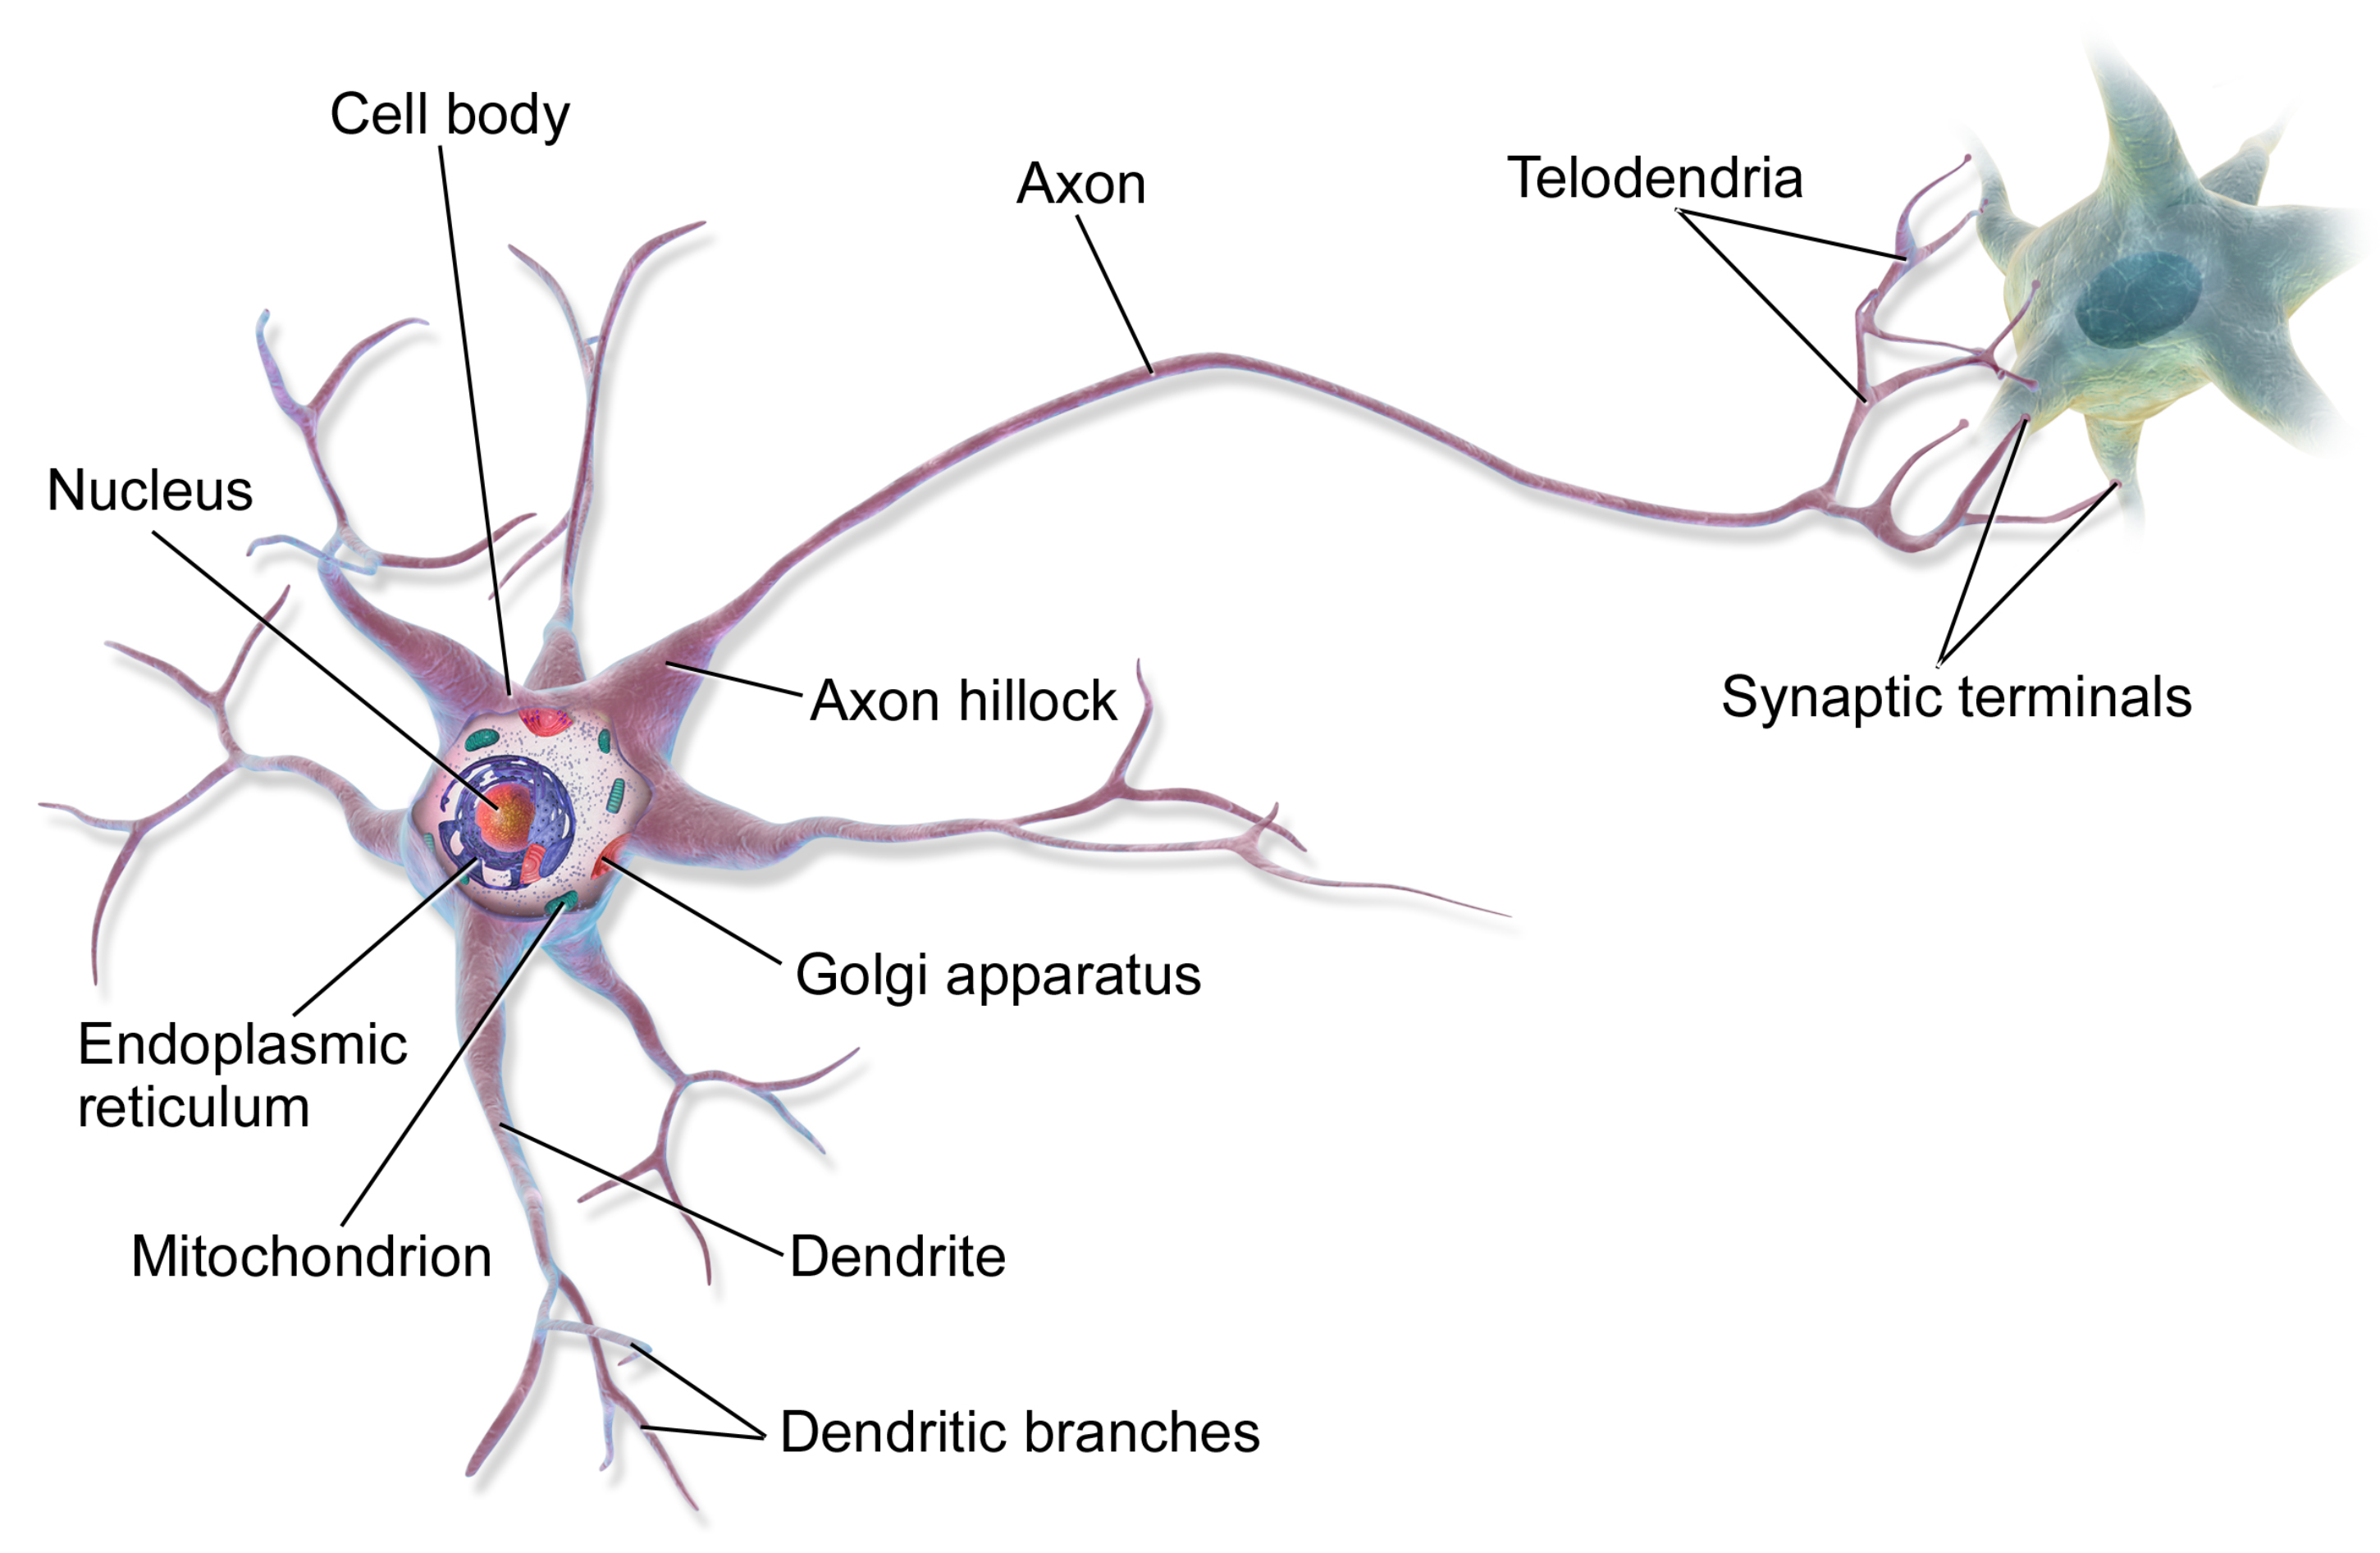
\includegraphics[width = 0.75\textwidth]{images/introduction/neuron_anatomy}
	 \def\c{Cartoon showing the basic anatomy of a neuron cell. }
	
	\caption[\c]{\label{fig:neuronanatomy} \c Of particular interest is the cell body (soma) and the protruding neurite (axon) which terminates on an adjacent cell body via a synaptic link provided by the dendrites. Figure adapted under a free to use license from the Wikipedia foundation \cite{neuronimage}.} 
\end{figure}
The morphology of neurons is a well-established and still active field of research \cite{Chen2012-qw} . There are a diversity of neuronal and dendritic structures each specialised to performing a particular task \cite{Squire2012-ru}.

This work will focus on the set of connections made in the superior colliculus by specialised neurones in the retina called retinal ganglion cells (RGCs). The superior colliculus in mice is a region of the midbrain which processes various sensory modalities, notably visual, auditory, and somatosensory information \cite{Seabrook2017-fa}.  In the superior colliculus there has not been an extensive classification of cell morphologies, although RGCs morphologies are well understood \cite{Ito2018-ef, Baden2016-kx, Gale2014-ss}. It is sufficient to consider that an RGC axon branches out into a relatively constrained and connected disk in its post-synaptic target area which can be seen in Golgi stains and microscopy studies of the mouse and related organisms \cite{Valverde1973-ws, Paxinos2014-kq}. It therefore has an ordered projective field and a continuous subset of the post-synaptic area has an ordered receptive field; see Section \ref{section:receptivefield}.

\subsection{Receptors and Ligands} \label{section:ephephrins}
Receptors are proteins, and ligands are molecules that have chemo-affinity with such proteins which is typically conferred by compatible binding domains \cite{noauthor_undated-od}. The Eph receptor is a tyrosine kinase protein that has an associated ligand called an ephrin both of which are membrane bound ensuring that cells physically contact during binding \cite{Beckmann1994-gx, Hirai1987-cx}. This class of molecules is ubiquitously expressed in many biological systems including the system of interest and are often involved in cell motility and guidance\cite{noauthor_undated-od}. Both Ephs and ephrins are able to signal, or interact, with other Ephs and ephrins and these interactions typically cause a cell to either experience an attractive or repulsive force based on relative levels of the available molecules. Most frequently two cells will express both Eph and ephrins and will therefore signal bidirectionally; see \cite{eph-ephrin-web}.
\begin{figure}[hb!]
	\centering
	\includegraphics[width = 0.75\textwidth]{images/introduction/eph-ephrin-binding}
	\def\c{Cartoon of a basic Eph-ephrin binding relationship. }
	
	\caption[\c]{\label{fig:ephrinbinding} \c Mutually compatible molecules come in physical contact on the cell membrane causing a reaction with some given affinity. Both the Eph and ephrin expressing cells receive a signal as a result of the reaction and the Eph expressing cell is said to receive the forward signal while the ephrin expressing cell is said to receive the reverse signal. Contact with the Eph-receptor by the ephrin ligand induces the forward signal in the Eph-receptor expressing cell. There are two major classes of Ephs and ephrins collectively referred to as A and B systems; within these systems there are many homologous molecules which have similar functions and can usually interact similarly with other molecules in the member class. The reaction can induce cell motility and this can be an attractive or repulsive movement and the repulsive actions are typically found in the A system while the attractive actions are found in the B system. Figure adapted under a free to use license from the Wikipedia foundation. \cite{ephrinimage}} 
\end{figure}
\subsection{Topographic Maps}
The final part of the fundamental biology to comment on is the notion of topographic maps. These are ubiquitous brain structures shared across multiple species and brain regions defined by an intuitive principle: physically neighbouring cells in some pre-synaptic region map to physically neighbouring cells in some post-synaptic region \cite{Swindale1996-kk, Cang2013-dw}. These maps a subset of the more general cortical map which share topological or continuous relations with multiple variables other than position e.g. direction and orientation selectivity for different stimuli \cite{Bednar2016-lg}. Most typically the topographic relationship is thought of as a one-to-one bijection which is a naturally intuitive notion, see Figure \ref{fig:topographicmap},  but there are some some salient and often ignored considerations.

\begin{figure}[h!]
	\centering
	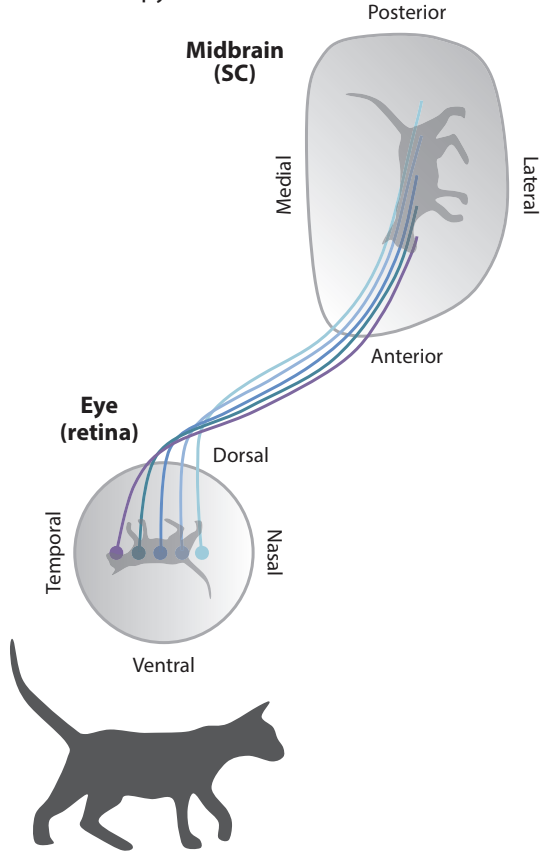
\includegraphics[width = 0.75\textwidth]{images/introduction/cartoon_topography}
	\def\c{Cartoon showing the retinotopic projection and relationship with the visual field. }
	\caption[\c]{\label{fig:topographicmap} \c Here a cat is presented as an image to a mouse's retina. This image is inverted by the lens of the eye and projected topographically into the SC where the neighbour relationships can be traced using the colour gradient. Figure adapted from Seabrook et. al. (2017) \cite{Seabrook2017-fa}.} 
\end{figure}
\subsubsection{Receptive and Projective Fields} \label{section:receptivefield}
The receptive field of a cell in the post-synaptic target is defined as the set of points in the stimulus field which the cell responds to \cite{Sherrington1906-et}; these are indicated by blue cones in Figure \ref{fig:projectivereceptivefield}. The projective field of a cell in the pre-synaptic target is the set of all points in the post-synaptic target that have synaptic contacts with that cell \cite{Lehky1988-nt}; these are indicated by the red cones in Figure \ref{fig:projectivereceptivefield}. These point based definitions can be natural extended to volumetric definitions by defining the projective/receptive field as the union of all point-wise fields in the area. 

\begin{figure}[h!]
	\centering
	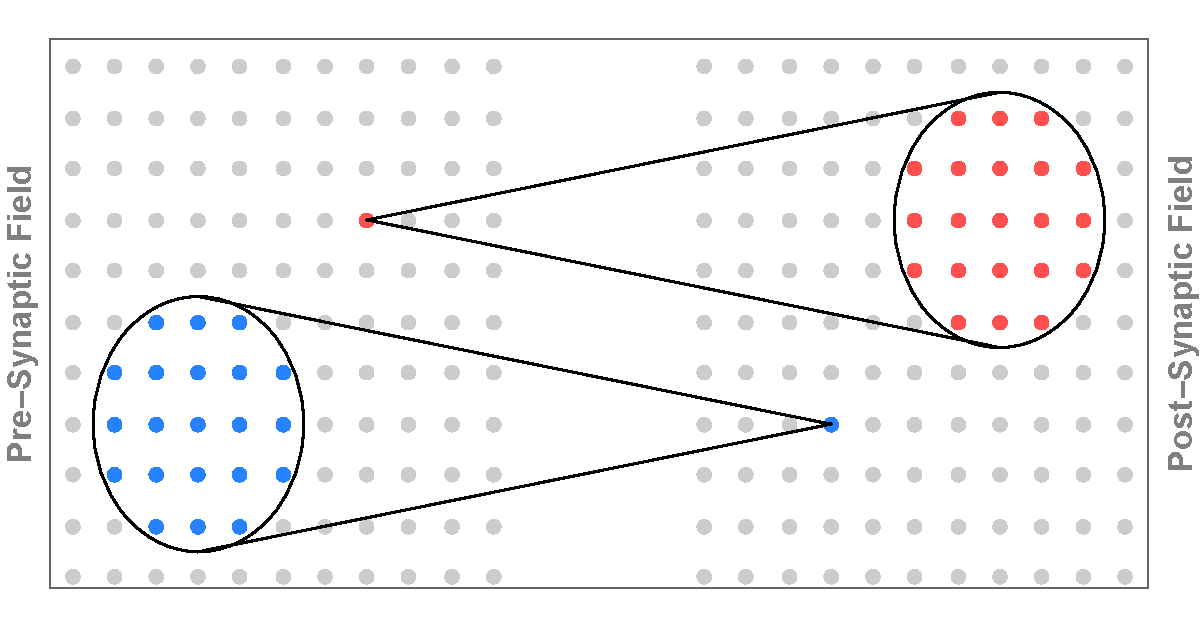
\includegraphics[width = \textwidth]{images/introduction/receptiveprojectivefields}
	\def\c{The pre-synaptic and post-synaptic fields are represented as ordered grids on the left and right respectively. }
	\caption[\c]{\label{fig:projectivereceptivefield} \c The receptive field is highlighted in blue with the blue node in the post-synaptic field responding to all blue nodes in the pre-synaptic field. The projective field is highlighted in red with all red nodes in the post-synaptic responding to the activation of the red node in the pre-synaptic field.} 
\end{figure}
If $f$ defines the projective field of a pre-synaptic point $i$ the mathematical definition is counter-intuitively the surjective map $f^\prime$ from the post-synaptic field to this point because function mappings cannot be many to one. This clarifies a problem with the discussion of projective and surjective fields: they are strictly not inverses of each other as the only way this is possible in a discrete context is for the map to be bijective. Each data source which attempts to detail these fields must be carefully analysed before conclusions are drawn.
\subsubsection{Dimensional Space of Developmental Topographic Mapping \label{sec:dimensionspace}}
The notion of projective and receptive fields can be unintuitive. It is generally easier to consider the topographic map as a function $W: \mathbb{R}^4 \rightarrow \mathbb{R}$ where $(x, y, \eta, \zeta) \mapsto w$, where $x$ and $y$ are coordinates in the pre-synaptic field, $\eta$ and $\zeta$ are coordinates in the post-synaptic field, and $w$ is the weight of the association between them. When considering development over a given timescale this definition can be extended to $(x, y, \eta, \zeta, t) \mapsto w$.
\section{Mouse Physiology, Anatomy, and Developmental Pathways}
The mouse retina has the geometry of a hemisphere (it is natural to represent it by a circular cross-section when it is flattened) and measures approximately 3mm in radius while the superior colliculus and adopts the approximate geometry of an ellipse with a greater diameter of approximately 2mm and a lesser diameter of approximately 1mm \cite{Park2012-yn, Seabrook2017-fa}. The superior colliculus of the mouse is located in the mid-brain and is organised in several different synaptic layers \cite{Ito2018-ef}. The superior colliculus acts to integrate and process multiple streams of sensory information as well as transmitting signals involved in movement: head shifting, escaping behaviour and freezing behaviours \cite{Ito2018-ef}. The inputs to the SC are varied with both external origin (e.g. retina) and inter-cortical origin (e.g. V1). This thesis is concerned with the organisation of the bundle of afferent neurons originating from the retina, specifically the RGCs, and terminating in the superficial layer of the SC; referred to as SC unless otherwise specified.
	
There are currently thought to be up to 42 different RGC types in the mouse retina with each of these thought to respond to specific elements of the visual field \cite{Goetz2022-ew, Baden2016-kx}. Each of the functions of these cell types will not be detailed but for further discussion about cell type classification, discussion, and potential issues see Sanes et. al. (2015) \cite{Sanes2015-xq}. A degeneracy amongst these cell types is now assumed and the pertinent mechanisms that guide them in forming a topographic map are considered rather than their ultimate cell fate. This simplifying assumption is legitimised by the fact ligand gradients are formed in the retina prior to RGC differentiation as will be made clear in the following discussion \cite{Marcus1996-kh}.

Cells in the retina and the SC express dual gradient and counter-gradients of Ephs and ephrins aligned along two characteristic orthogonal axes \cite{Marcus1996-kh, McLaughlin2005-jd, Lemke2005-iz}. The A system is arranged along the nasal-temporal (NT) axis in the retina and along the anterior-posterior (AP) or rostral-caudal (RC) axes in the SC. Here, EphA increases nasal-temporally and caudal-rostrally while ephrinA increases temporal-nasally and rostral-caudally. The B system is analogously arranged along the dorsal-ventral (DV) axis in the retina and the lateral-medial (LM) axis in the SC. Here, EphB increases dorsal-ventrally and medial-laterally while ephrinB increases ventral-dorsally and lateral-medially; see Figure \ref{fig:gradients}.

\begin{figure}[h!]
	\centering
	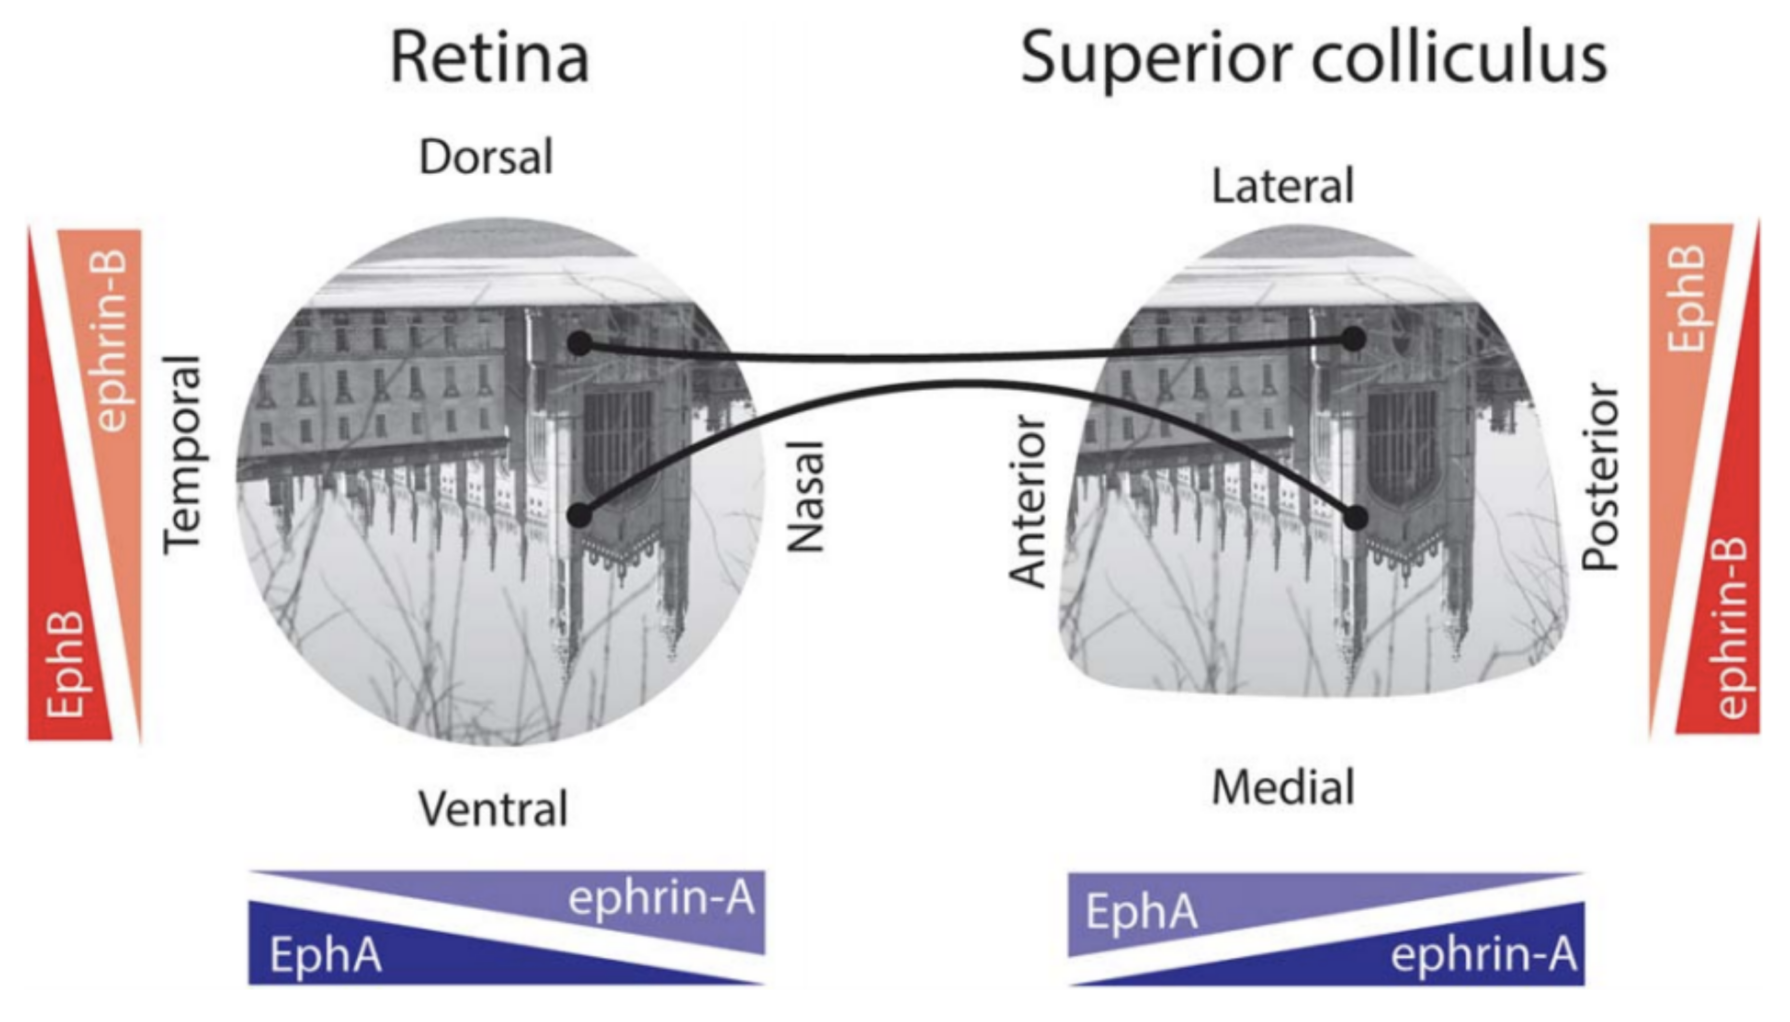
\includegraphics[width = 0.8\textwidth]{images/introduction/hjorth_gradients}
	\def\c{Each of the retina and SC have gradients and counter-gradients of EphA/B receptors and ephrin-A/B ligands with the A and B systems acting perpendicular to each other. }
	\caption[\c]{\c The chemotaxis then drives retinal locations to assigned SC locations preserving neighbour-neighbour relations through the graded expressions and establishing topography. Figure adapted from Hjorth et al. (2015) \cite{Hjorth2015-le}. \label{fig:gradients}} 
\end{figure}


The afferent neurons originating in the retina migrate towards the SC in a bundle passing through the optic chiasm where some pre-sorting is thought to occur \cite{Plas2005-yb}. Approximately 95\% of the afferents pass over the chiasm forming the contralateral projection into the SC and the remaining 5\% form the ispilateral projection \cite{Drager1980-px, Herrera2003-td, Koch2011-qz, Petros2008-rd}. The axon bundle makes a characteristic 90$^\circ$ turn before arrival at the SC. Each afferent then makes a characteristic overshoot of its eventual termination zone \cite{Yates2001-ug}. The overshoot is accompanied by interstitial branching into dendrites which, over time, are refined to a precise termination zone where the axon makes it final dendritic contacts \cite{McLaughlin2005-jd}. The termination zones typically occupy approximately $1$\% of the SC area \cite{McLaughlin2003-yy}. Each termination zone is defined by a characteristic location corresponding, in the wild-type, to a specific location of the visual field.

\section{Measurement and Data Analysis}

The modelling of the development of topography is driven by theoretical considerations but these are only relevant in the context of ground truth scientific data. These data will naturally be bound and constrained by the methods used to generate them and this section will detail some key data generation paradigms: surgical intervention, fluorescent dye focal injections, electrophysiology and multi-electrode arrays, calcium imaging, and intrinsic optical imaging.

\subsection{Microscopy}
Microscopy here will refer to fluorescence microscopy and can be subdivided into three distinct regimes: epifluorescence, confocal, and 2-photon. These three regimes are thought of as advancements of the same principle to produce higher quality images. Epifluorescence is the essential technique and relies on the principle of exciting a fluorophore with a wavelength that will cause it to fluoresce and measuring the emitted light. Confocal microscopy relies on the same emission principles as epifluorescence microscopy but uses a set of scanning mirrors and a pin-hole to improve the signal-noise ratio \cite{Inoue2006-rk}. Two-photon microscopy does not rely on the pinhole effect to generate in-focus images but rather the principle of two-photon absorption: two photons with roughly half the energy required to excite a fluorophore come together in a single quantum event and allow an emission photon \cite{Denk1990-ub}.

\subsection{Tracer Injections}
A tracer injection experiment injects a small amount of tracer material, typically DiI, into either the retina or the SC and allows it to diffuse into the opposing region \cite{Honig1989-by}. An injection diffusing from the SC to the retina is called retrograde, and from the retina to SC is anterograde. DiI is a compound which fluoresces and has the property that it diffuses laterally through the cell but not into other cells \cite{Sherazee2013-ky}. 

After a few days the retina and SC are removed and flattened and the amount of DiI is calculated through a microscopy measurement; see Figure \ref{fig:dii}. The resulting images then give a measure of the area of projection size to injection size and thus the ratio between two regions in the retrograde or anterograde projection can be calculated. Due to the diffusive nature of the procedure it is restricted to a limited region of either projection --- if multiple injection sites are used then the entire SC or retina will fill with DiI and no meaningful information can be gathered. This problem can be slightly mitigated by using DiI tags which fluoresce at different wave-lengths (green and red are typical) but this still limits the procedure to two injection sites; attempts to use more dyes have been thus far unsuccessful.

\begin{figure}[h!]
	\centering
	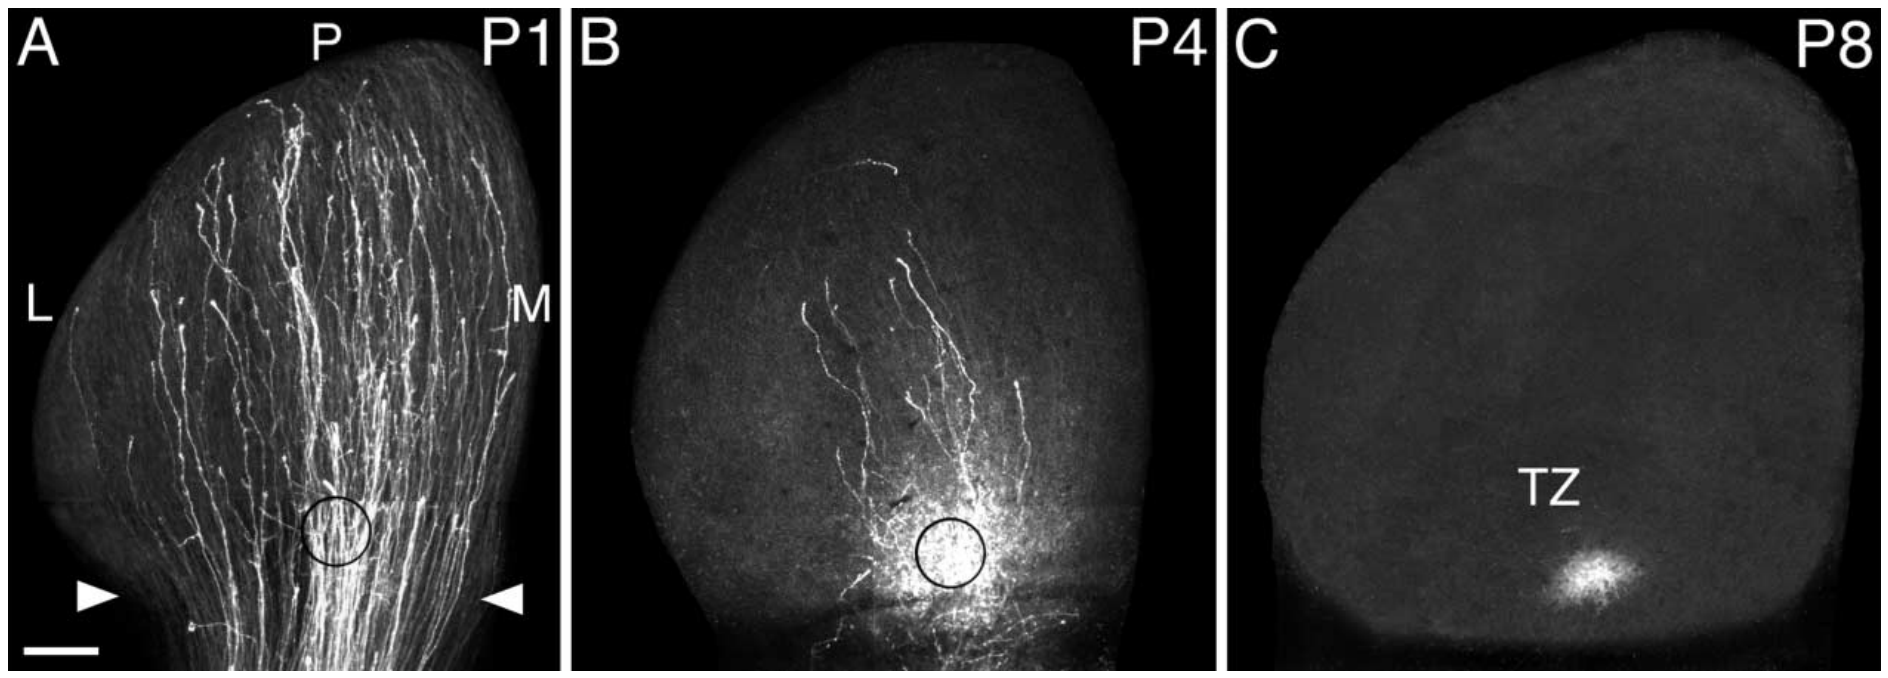
\includegraphics[width = \textwidth]{images/introduction/dii}
	\def\c{A typical experiment involving a series of DiI injections into the temporal retina at different developmental time points. }
	\caption[\c]{\label{fig:dii} \c The scale bar on the bottom left is $250\mu$m and the image covers the entire SC. The clarity of the image and the quality of the association with true anatomical features highlight the power of the DiI injection. The drawback is also highlighted because each injection at each time point represent a single pup that was killed to make the injection. Thus, no whole map can imaged from a single animal drastically reducing the conclusions that can be drawn about whole-map development. This problem is particularly pertinent in mutant studies where the map is drastically altered. Figure adapted from McLaughlin et. al. (2003) \cite{McLaughlin2003-yy}.} 
\end{figure}
\subsection{Calcium Imaging}
Calcium is used ubiquitously in biological systems as an intra-cellular and inter-cellular signalling mechanism. Notably, an influx of calcium in pre-synaptic terminals will trigger release of neurotransmitters and post-synaptically calcium transients appear to be key in mediating activity-dependent plasticity \cite{Grienberger2012-nr}. Therefore, calcium transients are a key indicator of cellular activity and can serve as a proxy for neuronal signalling. Calcium binds to several fluorescent proteins and these can be expressed in the specimen of interest  \cite{Grienberger2012-nr}. A microscopy technique can be used to stimulate the specimen over a time period and the changes in light intensity at a given location can be measured; see Figure \ref{fig:calcium}. The changes reflect the concentrations of calcium as the calcium binds to the available fluorophore and therefore the transient calcium levels in the specimen at the location of a given cell can be measured and used as a proxy for neural activity. 

\begin{figure}[h!]
	\begin{subfigure}{0.3\linewidth}
		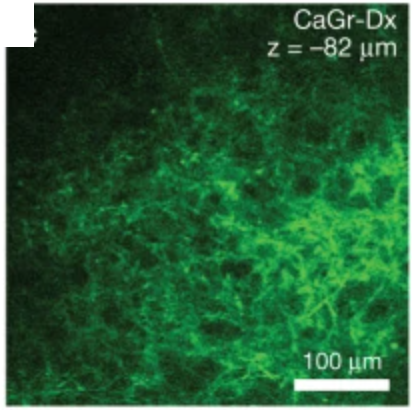
\includegraphics[width = \textwidth]{images/introduction/calcium1}
		\caption{} 
	\end{subfigure}
~
	\begin{subfigure}{0.4\linewidth}
		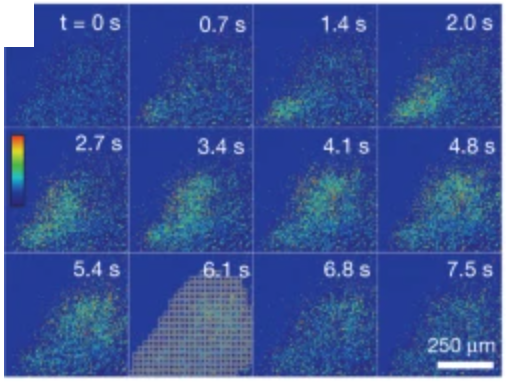
\includegraphics[width = \textwidth]{images/introduction/calcium2}
		\caption{} 
	\end{subfigure}
~
	\begin{subfigure}{0.2\linewidth}
		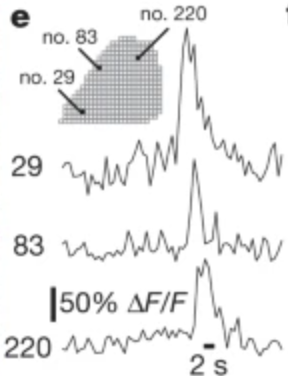
\includegraphics[width = \textwidth]{images/introduction/calcium3}
		\caption{} 
	\end{subfigure}
	\def\c{A series of images detailing the transient calcium imaging procedure. }
	\caption[\c]{\c First, confocal microscopy is used to image a small patch of the superior colliculus which has been tagged with a green fluorescent protein; (a). This imaging is performed over an extended time period and the intensity of the fluorescence is measured at every pixel of the image allowing for calcium transients to be recorded; (b). These transients can be examined at each location and give a proxy for neural activity and they may, for example, be associated with spiking events; (c). Figures reproduced from \cite{Ackman2012-uu}. \label{fig:calcium}}
\end{figure}


\subsection{Intrinsic Optical Imaging \label{sec:optical}}
The intrinsic optical imaging method uses a continuous periodic stimulation along which is then combined with concurrent passive activity recording to develop a map of mouse retinotopy \cite{Kalatsky2003-cz}. The advantage is that, while traditional methods rely on an input-output approach, this passive periodic recording allows systematic effects, errors, and noise to be averaged out.

The stimulation is provided to one eye by a small monitor presenting a single bar tracking in a horizontal or vertical fashion. The phase of the bar encodes the location in the visual field. The cortex is imaged using infra-red stimulation and recording through a charge-coupled device. The images are binned in time and the biological artefacts, such as the haemodynamic response, are removed by Fourier decomposition. This involves choosing a period of stimulation sufficiently different to known internal rhythms and selecting the harmonics with highest amplitude corresponding to the frequency of the drift grating. After this data is processed the response times of a location in the cortex is measured and due to the forward-reverse pattern of stimulation there will be two natural responses $s$ and $T-s$ for a period length $T$. These can be added and averaged to find the delay time of the system which should be uniform across the map, or subtracted and averaged to find the phase (visual field location) associated with that particular cortical region \cite{Kalatsky2003-cz}. In this fashion a whole map recording is made with some precision of a single specimen. These details are summarized in Figures \ref{fig:ois1} and \ref{fig:ois2}.
\begin{figure}[h!]
	\centering
	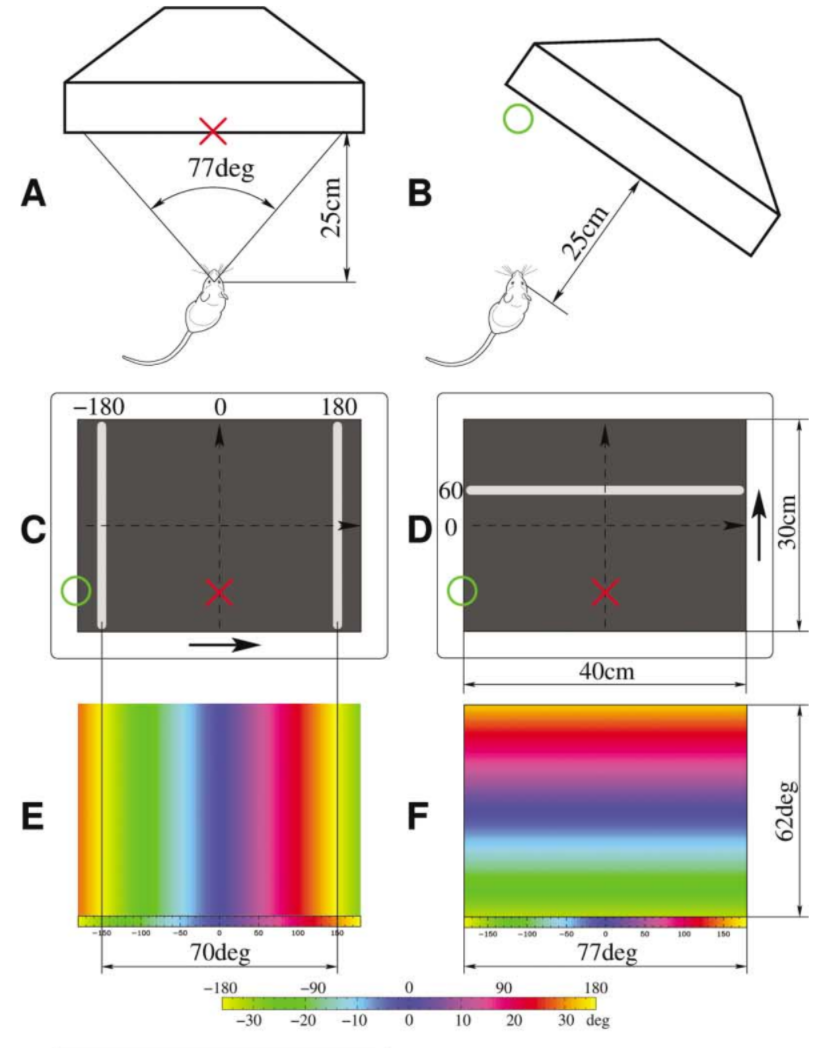
\includegraphics[width = 0.7\textwidth]{images/introduction/kalatsky_experiment}
	\def\c{The experimental procedure is detailed showing first the correct positioning of the stimulus screen for an ispilateral and contralateral stimulation (A) or a purely contralateral stimulation (B). }
	\caption[\c]{\label{fig:ois1}  \c The stimulus is presented as a series of horizontally (C) or vertically (D) drifting bars to measure azimuthal and elevational responses. The phase associated with each bar is mapped onto the colour schemes presented in (E) and (F). Figure adapted from Kalatsky and Stryker (2003) \cite{Kalatsky2003-cz}}
\end{figure}

\begin{figure}[h!]
	\centering
	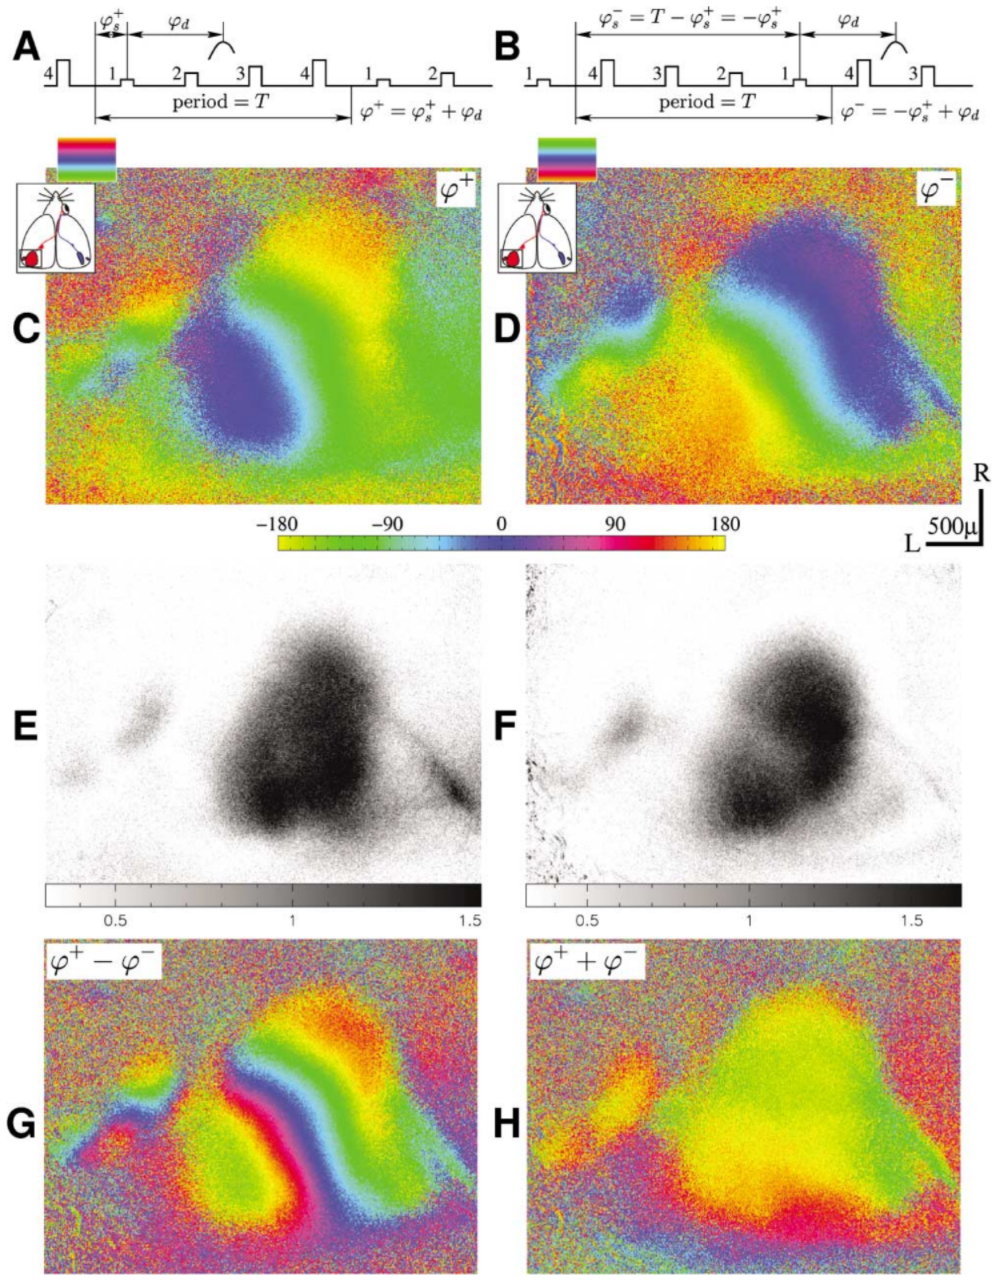
\includegraphics[width = 0.7\textwidth]{images/introduction/kalatsky_phase}
	\def\c{The experimental result is presented where forward drifting (A) and reverse drifting (B) bars are presented to measure the azimuthal response. }
	\caption[\c]{\label{fig:ois2}  \c The phase recordings for each of these stimuli are presented directly below in (C) and (D) and the bulk responses are presented in (E) and (F). The phase-delay trick is used to remove the haemodynamic response by subtracting the two phases giving the complete map in (G) and confirming a mostly uniform phase across the colliculus by adding the two phases and thus validating the method. Figure adapted from Kalatsky and Stryker (2003) \cite{Kalatsky2003-cz}.}
\end{figure}

\subsection{Electrophysiological recording}
Electrophysiological recording aims to make measurements of the electrical environment of a neuron at a given location, typically voltage, to understand the electrical activity of a cell. This can be translated into spike trains of action potentials which are of interest to understand the signalling relationship between two independently recorded locations.

The recording is made through an electrode which may record the activity at the membrane of a single neuron (single-unit) or multiple neurons (multi-unit). This may be done \textit{in vivo} or \textit{in vitro}. In a single electrode setup the receptive field of a neuron in the colliculus may be measured by stimulating various parts of the retina. This stimulation can be performed via visual stimulation (presentation of a visual image or scene), or via another electrode which stimulates a portion of the retina \cite{Boulton1990-ff}.

Multielectrode Arrays (MEAs) follow the same principle as single electrodes excepting that many channels/electrodes record simultaneously. This confers the advantage of regular sampling of a biological region with concurrent recording \cite{Potter2001-lg}. In this fashion broader statements about correlated regions over the colliculus can be made and more complicated phenomena with spatio-temporal characteristics, such as retinal waves, can be observed.
\subsection{Lattice Method \label{sec:lattice}}
While it is relatively straightforward to establish a feed-forward, or feed-backward association from any point in the pre-synaptic field or post-synaptic field it is relatively difficult to assess the quality of a map made from a collection of associations. Due to the complex nature of biological topographic maps whole-map analysis is often not performed. The Lattice Method is an algorithm designed to assess map quality in both forward and reverse directions \cite{Willshaw2014-ms}. The algorithm attempts to make a topographic matching between a pre-synaptic and post-synaptic field. First, the direction of the map is chosen by specifying which field is the image and which is the pre-image under the mapping: post-synaptic pre-image to pre-synaptic image or vice-versa. Second, a desired target spacing is specified and a selection of $N$ nodes from the all available points in the pre-image is made randomly in the following subroutine: chose a random unselected point and retain it if the spacing with already selected nodes exceeds the minimum spacing; if $N$ suitable nodes cannot be found after 10000 trials then restart the subroutine with the target of $N-1$ nodes. Once a selection of nodes has been made in the pre-image create a Deluaney tiling is made on the points defining these nodes \cite{Lee1980-wr}.  Each node in the pre-image is associated with a number of locations in the image given by the measured mapping. A bijection between the pre-image and image is created by associating each selected node in the pre-image with the average location of all points in the image it projects to. The edges of the Deluaney tiling are mapped under this bijection to create a graph in the image and any nodes attached to edges in the image-graph that intersect are removed to create a subgraph. The subgraph defines a well-ordered topographic mapping and the bijection restricted to this subgraph is a perfect topographic map. This procedure is summarised in Figure \ref{fig:lattice_procedure}. If the map is smoothly continuous then the amount of edges removed should be zero. Since the mapping is typically discrete there will be some removal of edges and the fraction of removed nodes gives an indication of the quality of the map.
\begin{figure}[h!]
	\centering
	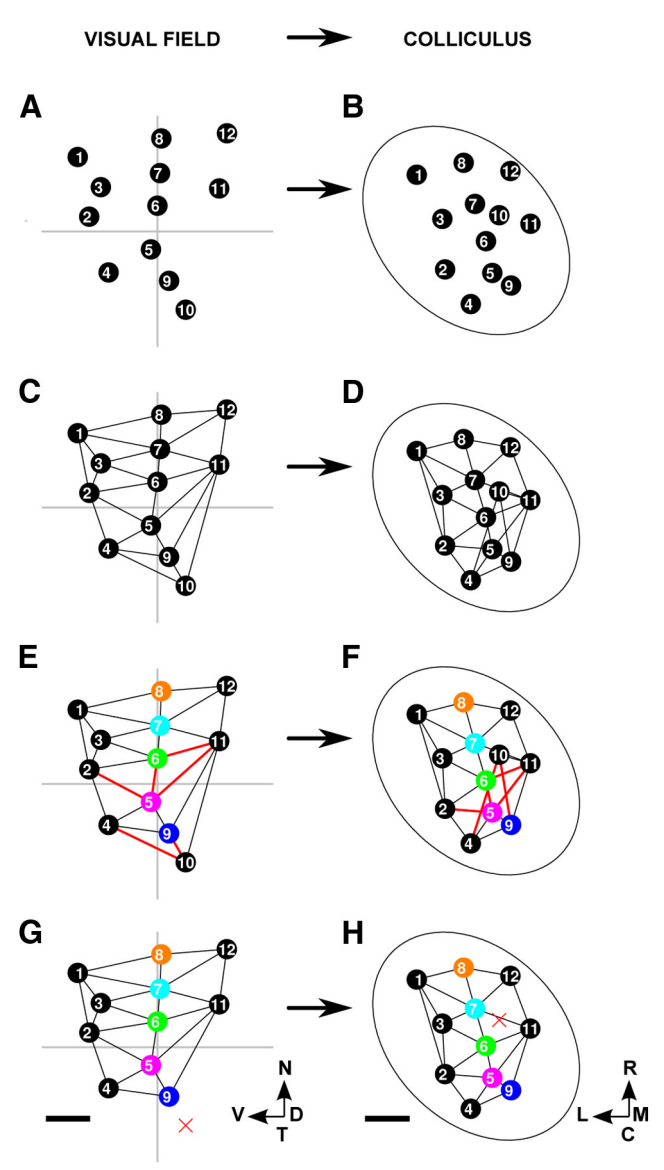
\includegraphics[width =0.6\textwidth]{images/introduction/lattice_procedure}
	\def\c{The method for creating a map with the visual field as the pre-image. }
	\caption[\c]{\label{fig:lattice_procedure} \c The points in (A) are first chosen according to the random sampling routine described in Section \ref{sec:lattice}. These are then mapped into the colliculus by finding their average synaptic location (B). A Deluaney tiling is made on the pre-image in the visual field (C) and the edges are placed on the nodes in the colliculus (D) under the same mapping as the points. Edges that are crossing in the image are identified and labelled in red (F) and mapped back into the pre-image (E). These edges are removed to give the largest submap with perfect topographic order (G-H). Varying the number and location of points in the pre-image can be used to determine map quality and reveal salient features of regular, but not wild-type, maps. Figure adapted from Willshaw et. al. (2014) \cite{Willshaw2014-ms}.} 
\end{figure}

It is important to note that $f: X \rightarrow Y$ and $g: Y \rightarrow X$ for arbitrary $g, f$ does not imply that $f^{-1} = g$. The Lattice Method therefore gives the quality of both the forward mapping as well as the reverse mapping between the pre-synaptic and post-synaptic fields. Figure \ref{fig:lattice_results} shows the Lattice Method applied to a wild-type mouse in forward and reverse directions.
\begin{figure}[h!]
	\centering
	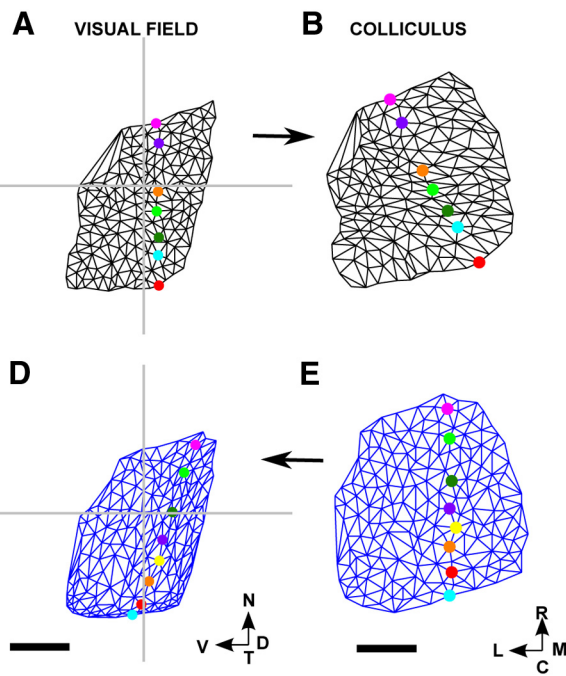
\includegraphics[width = 0.6\textwidth]{images/introduction/lattice_results}
	\def\c{The method can be applied with the visual field or colliculus as both the pre-image and the image respectively. }
	\caption[\c]{ \c Both maps constructed from optical image scanning of a wild-type mouse are shown in the right panel. The visual field as the pre-image is detailed in black,  and as the image in blue. A coloured code slice of the function is highlighted with a selection of nodes and the colouring reflects the topographic continuity. Figure adapted from Willshaw et. al. (2014) \cite{Willshaw2014-ms}. \label{fig:lattice_results}  }
\end{figure}

\FloatBarrier
\section{Mutant Mouse Observations}
The scientific understanding of the development of the retinotopic system, and indeed a large part of developmental biology, has been accelerated by genetic mutation studies; see section \ref{section:genemutations}. Several recent genetic manipulations that have been performed in mouse and their effects on the organisation of the topographic organisation will be detailed here and their theoretical implications of their observations discussed Section \ref{section:developmentaltheory}.
\subsection{Ephs and Ephrins}
In the case of the mouse retinotopic system there are two systems, labelled A and B, of Ephs and ephrins that are expressed in a gradient along orthogonal axes of the retina and the SC respectively, allowing for this bidirectional signalling to occur; see Figure \ref{fig:ephrinbinding}. The A and B systems are thought to have different interactions and are most often thought to act independently of one and other; for a summary of these interactions see Table \ref{table:ephephriniteraction}. A series of studies has confirmed the existence of several classes of both A and B molecules and these are thought to interact in similar ways; the interaction properties of these subclasses are assumed to be degenerate. The gradients for the A system along the retina have been measured by and shown to follow a complementary pattern where the Ephs decrease in tandem with the increase of the ephrins \cite{Reber2004-wq}. This gradient-counter-gradient pattern was shown to be repeated in the SC allowing for bidirectional signalling to occur along the two axes. Interestingly, the B system is also expressed at the optic chiasm where the incoming retinal axon bundle diverges into the contralateral and ispilateral portions of the brain \cite{McLaughlin2003-co}.
\begin{table}
	\centering
	\begin{tabular}{|c|c c c c|}
		\hline
		\textbf{Molecular Type} & EphA & EphrinA & EphB & EphrinB \\
		\hline
		EphA & Attractive & Repulsive & None & Cross-talk* \\
		EphrinA & Repulsive & Attractive & None & None \\
		EphB & Cross-talk* & None & Repulsive & Attractive \\
		EphrinB & None & None & Attractive & Repulsive \\
		\hline
	\end{tabular}
	\def\c{A brief summary of the interaction properties of each of the major classes of Ephs and ephrins in the developing mouse retinotopic system. }
	\caption[\c]{\c Generally, the interactions between Ephs and ephrins is context dependent: they may be attractive, repulsive, or bifunctional; see Section \ref{section:ephephrins}. It should be noted that while much work has been done to establish the function of the EphA-ephrinA relationship there has been less work done on the EphB-ephrinB relationships or on the potential interaction between classes \cite{Lemke2005-iz}. EphA4 has been observed to bind with all ephrinBs and EphB2 can bind to ephrinA5 indicating a limited amount of cross talk between the two classes \cite{Gale1996-zd, Himanen2004-jj}. \label{table:ephephriniteraction}}
\end{table}
There are currently 14 identified classes of Eph receptors and 9 classes of associated ephrin ligands. These classes are subdivided into 8 classes of EphA receptors, 6 classes of EphB receptors, 6 classes of associated ephrin-A ligands, and 3 classes of associated ephrin-B ligands. The interaction of the tyrosine-kinase protein and its associated ligand is mediated by proximity: the ephrins are membrane bound and the Eph receptors will be stimulated by contact with this membrane. The receptor-ligand pairing occurs within all subclasses of an A/B grouping, but their does not appear to be interaction between A and B pairs with the exception of EphA4 which can bind to both ephrinAs and ephrinBs and EphB6 which can bind to ephrinA5 \cite{McLaughlin2005-jd, Lemke2005-iz, Gale1996-zd, Himanen2004-jj}.

The expression of these molecules is graded through both the retina and SC with the A and B classes being expressed perpendicular to each other. In mouse the retina expresses EphA5 and EphA6 in an increasing fashion from the nasal to temporal locations, EphA4 is expressed in an ungraded fashion (constant expression) across the retina, ephrin-A2 and ephrin-A5 are expressed in a decreasing fashion from nasal to temporal locations, EphB1-B4 and EphA6 are expressed in an increasing fashion from dorsal to ventral locations, ephrin-B1 and ephrin-B2 are expressed in a decreasing fashion, and ephrin-B3 is expressed in an ungraded fashion across the retina  \cite{McLaughlin2005-jd, Lemke2005-iz}. In the SC the EphA4, EphA3, and EphA7 are expressed in a decreasing fashion from the anterior to posterior locations, ephrinA2 is expressed in an increasing fashion anterior to posterior but then decreasing towards the final posterior locations, EphB1-B3 are expressed in a decreasing fashion from lateral to medial locations, and finally ephrin-B1 is expressed in an increasing fashion from lateral to medial locations. These gradients are summarised graphically in Figure \ref{fig:measuregradients}. The promiscuity of the various subclasses means that they are thought of as linearly additive resulting in a total gradient and counter-gradient in both orthogonal directions of both the retina and the SC. The graded expressions guarantee that for each position in the retina there is a unique position in the SC where chemotactic forces are balanced in all directions: the topography emerges from guidance to this position. This information is summarised previously in Figure \ref{fig:gradients}.

\begin{figure}
	\centering
	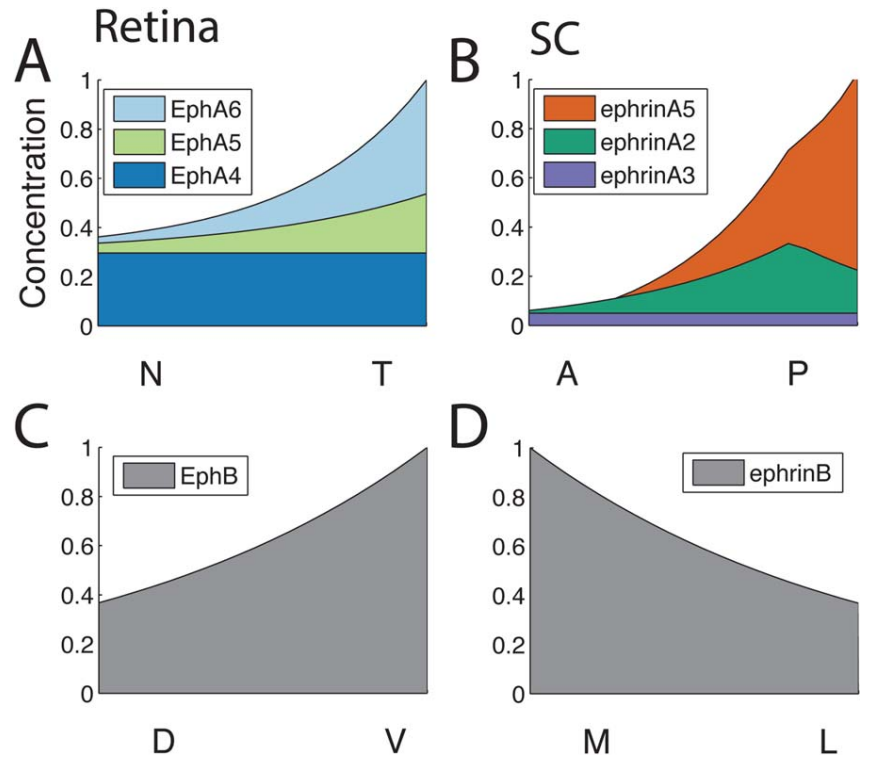
\includegraphics[width = 0.5\textwidth]{images/introduction/gradientsEphEphrinMeasured}
	\def\c{A cartoon of the primary gradient expression profile in the A and B systems in the superior colliculus and retina. }
	\caption[\c]{\label{fig:measuregradients} \c The A system has been measured by proxy of mRNA expression and the contribution of each subclass is coloured and displayed in (A) and (B). The EphA family generally has an exponential profile increasing from nasal to temporal regions of the retina with the exception of EphA4 which is expressed as a constant. The ephrinA family generally has an exponential profile increasing from anterior (rostral) to posterior (caudal) regions of the colliculus. The B system has few measurements available and is shown in grey in (C) and (D). The EphB  family is assumed to have an exponential profile increasing from the dorsal to ventral regions of the retina. The ephrinB family is assumed to have an exponential profile increasing from the lateral to medial regions of the colliculus. Figure adapted from Hjorth et. al. (2015) \cite{Hjorth2015-le}.}
\end{figure}
\begin{figure}
	\centering
	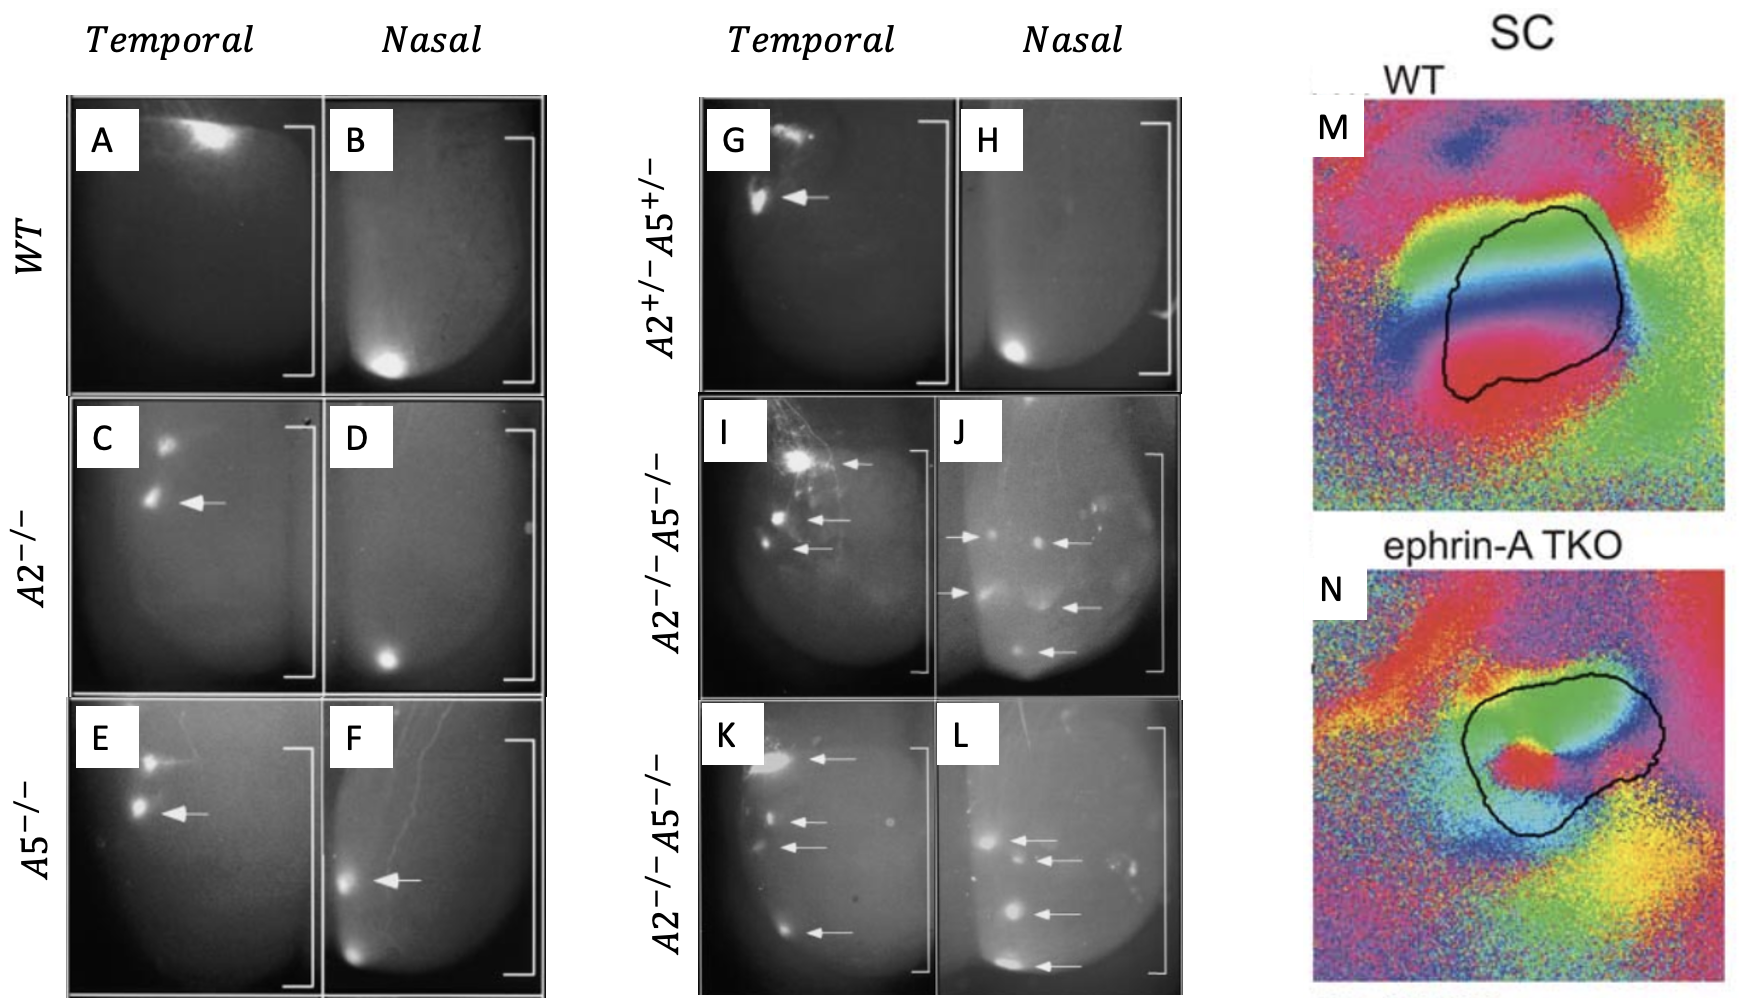
\includegraphics[width = 0.8\textwidth]{images/introduction/ephrinKO}
	\def\c{The effect of multiple combinations of single and double ephrinA2, ephrinA5, and ephrinA3 knock-outs. }
	\caption[\c]{\label{fig:ephrinknock-outs} \c A DiI injection is performed for wild-type (A and B), ephrinA2 double knock-outs (C and D), ephrinA5 double knock-outs (E and F), and ephrinA2A5 single knock-outs (G and H) while two examples of ephrinA2A5 double knock-outs are shown in (I-L). It can be seen that the double knock-out of ephrinA2 induces ectopic projections in the temporal retina while the double knock-outs of ephrinA5 induces ectopic projections across the whole NT. The single knockout of both ephrinA2 and ephrinA5 induces ectopic projections only temporally but these ectopic have less precisely defined projection zones. The double knock-out of ephrinA2A5 induced multiple ectopic projections across the entire NT-AP axis. The whole map in the ephrinA2A3A5 triple knock-out elevational and azimuthal scans are presented in M and N respectively. These reveal the disorder but notably demonstrates that there are still localised functional domains. Figures (A-L) adapted from \cite{Feldheim2000-ec}. Figures M and N adapted from \cite{Cang2008-ez}.}
\end{figure}
\subsection{EphrinA knock-outs}
One natural way to test the role of an Eph/ephrin is to knockout a component and observe the effect on topographic map formation; knockout experiments have been performed extensively in the context of the ephrinA system. These are the single knockout, double knockout, and triple knockout studies: ephrinA2 and ephrinA5 (single), ephrinA2A5 (double), and ephrinA2A3A5 \cite{Frisen1998-jw, Feldheim2000-ec, Cang2008-ez}. The effect of these is to largely disrupt the mapping along the NT-AP axis. EphrinA2 makes its primary contributions to the total ephrin gradient in the anterior colliculus, and accordingly in the ephrinA2 knock-down topographic order along this axis is primarily lost anteriorly. Similarly, the ephrinA5 contribution is most significant in the posterior colliculus and the ephrinA5 knock-down phenotype has a loss of order in this region. The ephrinA2A5 knockout combines these effects presenting a loss of order along the entire AP axis with multiple ectopic projections being observed for single retinal injection sites; see Figure \ref{fig:ephrinknock-outs}. The ephrinA2A3A5 knockout is similar, but the effect appears to be more pronounced with optical image scans showing a lack of order along the AP axis. Interestingly, some topographic order is preserved and the maps are not comparable to a random association between points on the AP and NT axes \cite{Willshaw2014-ms}. 


\FloatBarrier
\subsection{EphA3 knock-in \label{sec:epha3}}
The EphA3 knock-in involves inserting a non-endogenous Eph receptor in the Islet2 region of the mouse genome \cite{Brown2000-da, Reber2004-wq}. This insertion is particularly interesting because this region is only expressed in approximately 40\% of retinal cells and is not expressed in the SC \cite{Brown2000-da}. The expression pattern along the retina is often referred to as ``salt-and-pepper" suggesting that $Islet2^{+/-}$ cells are distributed randomly, but there is little work to formally establish the distribution \cite{Lemke2005-iz}. The addition of a constant amount of EphA3 to a fraction of RGCs induces an ectopic projection in the mapping into the SC but unlike the ephrinA knock-outs these ectopics have a stereotypical location which they project to; see Figure \ref{fig:epha3anatomical}. The heterozygous knock-in has ectopic projections from nasal regions in the retina but these collapse in temporal regions; see Figure \ref{fig:epha3collapse}B. The homozygous knock-in has a stereotypical ectopic projection for every point in the retina with no collapse point which creates a complete duplication of the topographic map both anatomically and functionally see Figures \ref{fig:epha3anatomical}, \ref{fig:epha3collapse}C, and \ref{fig:epha3functional}. This is most prominent in the double knock-in where there are therefore two complete representations of the visual field in the neural space occupied by the SC. It has been claimed that the $Islet2$ expressing and non-expressing cells are perfectly partitioned into the anterior colliculus (wild-type) and posterior colliculus (EphA3) \cite{Cang2013-dw}. 

\begin{figure}[h!]
	\centering
	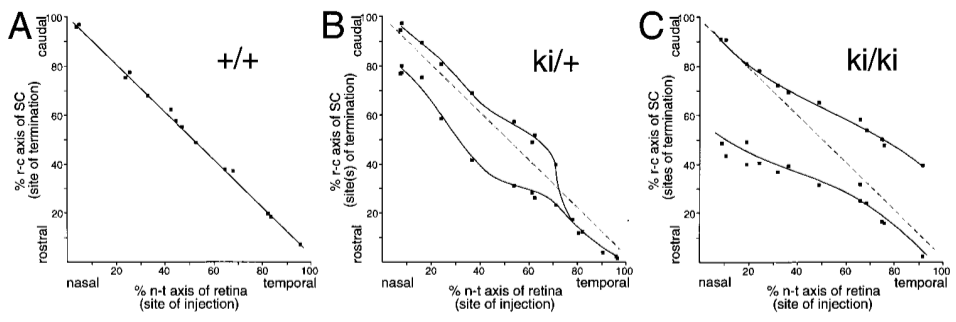
\includegraphics[width = 0.6\textwidth]{images/introduction/brownEphA3}
	\def\c{Bulk anatomical tracer experiments on the EphA3 knock-in mutant.}
	\caption[\c]{\label{fig:epha3collapse} The data points in each of the panels represent the location of the centres of tracer injection at a given retinal location.  The wild-type injections shown in panel A form a predictable straight line indicating an ordered topography. The heterozygotes shown in panel B have two projections in the nasal portion of the retina but these collapse to form a single projection as the injection site moves toward the temporal retina. The homozygotes shown in panel C also exhibit the stereotypical ectopic projection and there is no collapse point indicating the presence of two ordered topographic maps.  Figure adapted from \cite{Brown2000-da}.}
\end{figure}


\begin{figure}
	\centering
	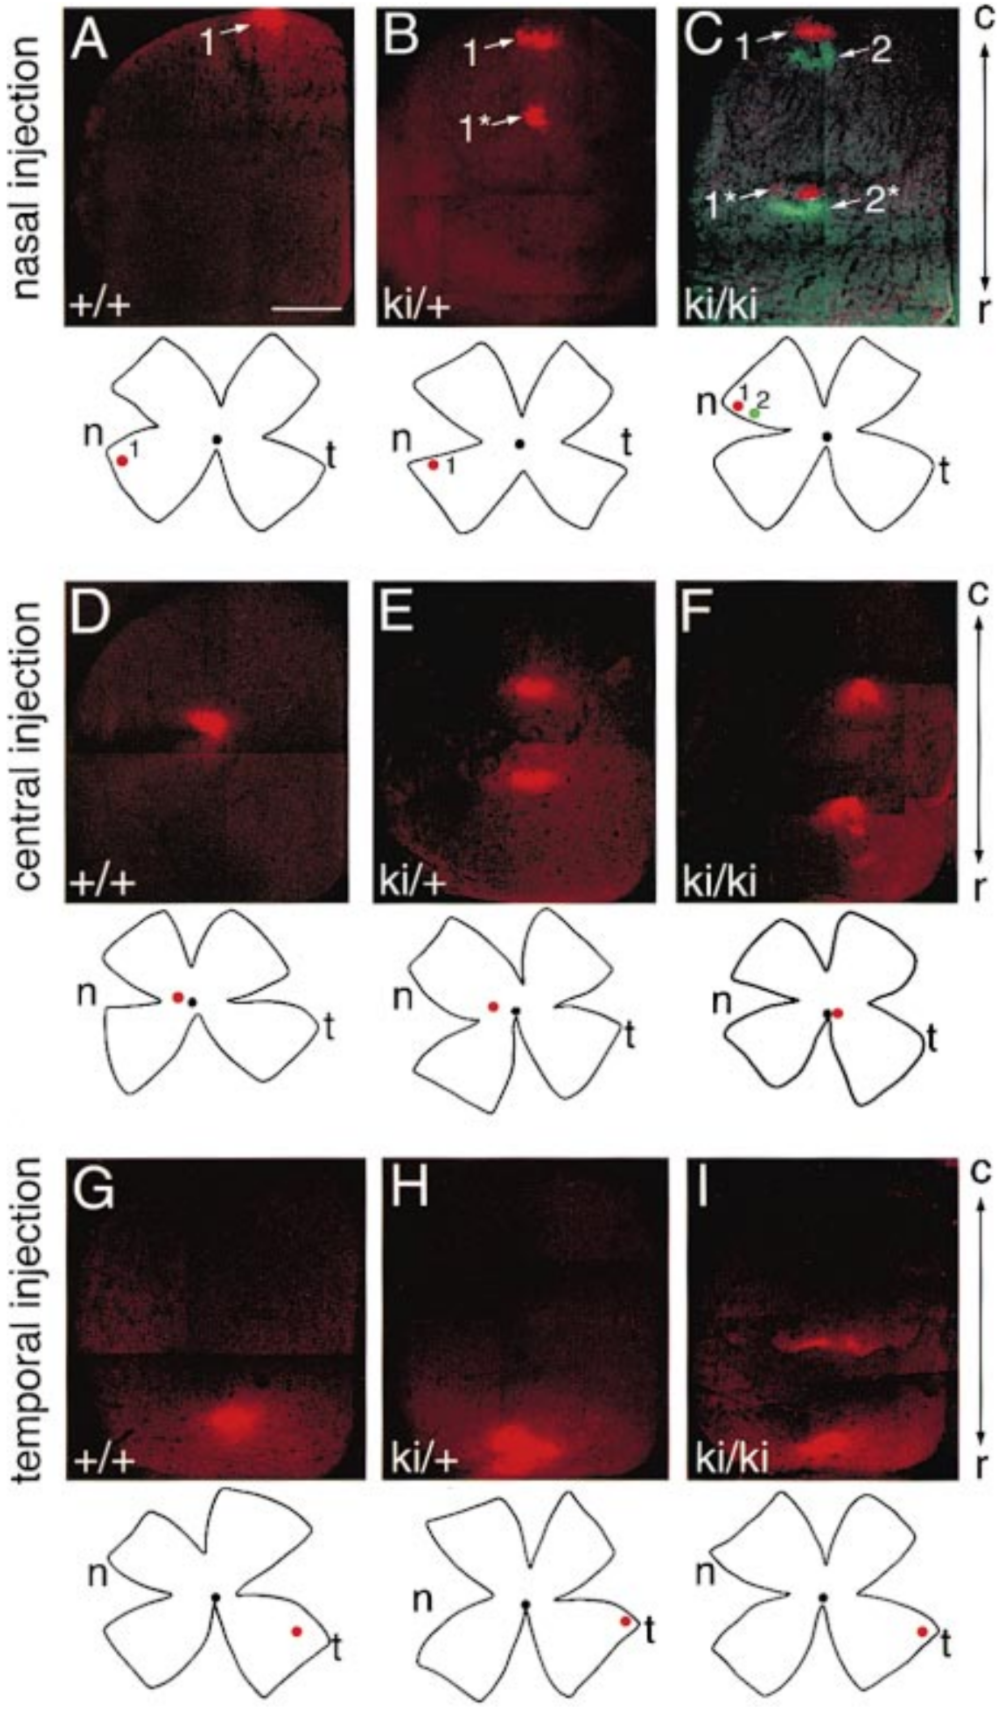
\includegraphics[width = 0.6\textwidth]{images/introduction/epha3anatomical}
	\def\c{Visualisations of the wild-type, heterozygous, and homozygous EphA3 knock-in mice. }
	\caption[\c]{\label{fig:epha3anatomical} \c An anterograde injection is made in the nasal, central, and temporal retina for a wild-type, heterozygous EphA3 knock-in, and homozygous EphA3 knock-in in the left panel (a). The heterozygote presents a duplicated projection in the caudal (posterior) and central regions but just one projection in the rostral (anterior) region. The collapse point of the map is where the two distinct mappings coalesce into a single mapping which can be seen in (B) at the 75\% tick of the NT axis. The homozygote has duplicated projections in all three regions. Two injections with different fluorescent tags are performed nasally in the homozygote demonstrating that the two projections maintain relative ordering. Figure adapted from \cite{Brown2000-da}.}
\end{figure}

The heterozygote is of particular interest. The anatomical collapse points in this mutant appear to have more variation than in the homozygote. Furthermore, the visual field maps produced by heterozygous specimens have widely varied visual characteristics which have been conjectured to arise from a stochastic interaction between chemotactic and activity-based development mechanisms \cite{Owens2015-zv}. Attempts have been made to categorise these variations but they have been inconclusive due to mathematical considerations of the methodology used, as well as labelling discrepancies in the data. Nevertheless, these specimens are a prime data-set to develop insights about the development effect of this mutant as well as generate and validate hypotheses from theoretical considerations. 

\begin{figure}
	\begin{subfigure}{0.625\textwidth}
		\centering
		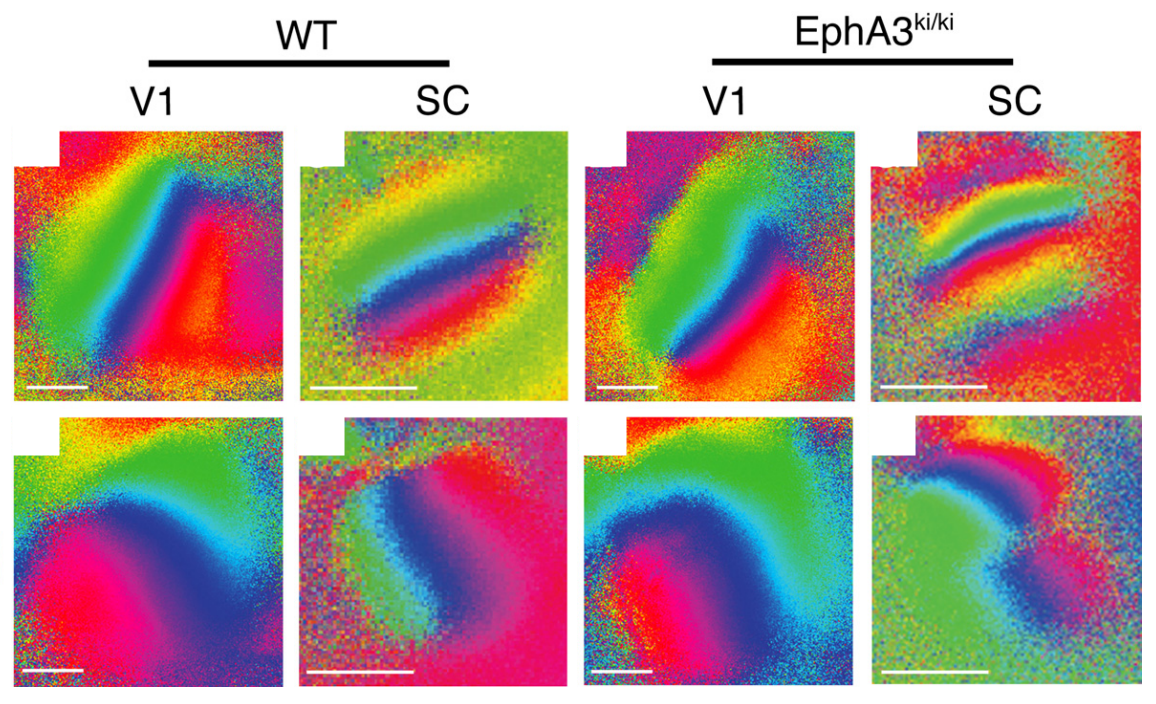
\includegraphics[width = \textwidth]{images/introduction/epha3hom}
		\caption{}
	\end{subfigure}
~
	\begin{subfigure}{0.375\textwidth}
		\centering
		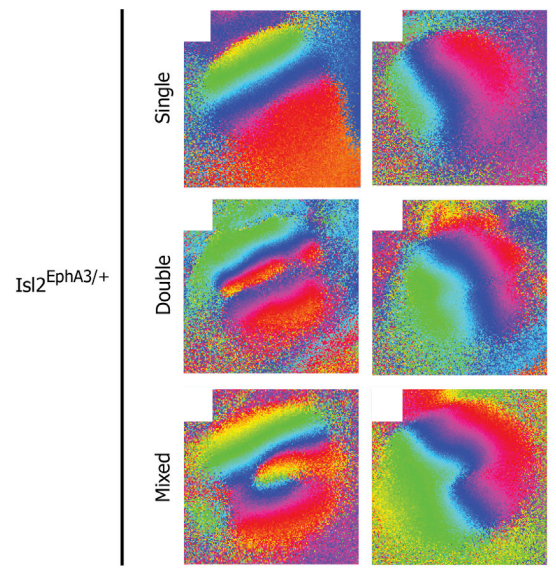
\includegraphics[width = \textwidth]{images/introduction/epha3het}
		\caption{}
	\end{subfigure}
	\def\c{Intrinsic optical imaging scans of EphA3 knock-in mice. }
	\caption[\c]{\label{fig:epha3functional} \c A functional map of the wild-type and the homozygous EphA3 knock-in is presented in the left panel (a). Both maps show functional continuity and a near complete representation of visual space but strikingly the EphA3 knock-in has two such representations completely contained in posterior and anterior regions. The duplication only occurs along the AP axis and the map is singular in the DV axis. Shown here are both the superior colliculus and V1 and interestingly V1 does not present this duplication. Figure adapted from \cite{Triplett2009-si}. \\\\
	The heterozygote maps also have a representation of functional space but they are more varied and less ordered. These maps appear to occasionally present a complete duplication of visual space like a homozygote, occasionally a single representation like a wild-type, and occasionally something in between labelled here as ``mixed". Further analysis on these variants is required.  Figure adapted from \cite{Owens2015-zv}.}
\end{figure}
\FloatBarrier
\subsection{Neural Activity}
The organisation of synaptic connections via activity driven plasticity has notionally existed in the literature since at least the introduction of the chemo-affinity hypothesis as an alternative theory to chemotactic based wiring \cite{Chung1974-oy}. It is difficult to summarise the basic principles of organisation without reference to a computational or mathematical model but it is postulated that a topographic map can be formed by modifying (or creating) a set of synapses with a Hebbian rule and an abstract form of neural activity in the pre-synaptic and post-synaptic regions. The Hebbian rule  states that neurons that are persistently co-active will form synapses such that the potentiation of one leads to the potentiation of another \cite{Abbott2000-gl}. It appears that the activity does indeed propagate forward from the retina into the SC and is spatiotemporally correlated \cite{Ackman2012-uu}.

\subsubsection{Three Periods of Distinct Waves}
There appear to be three periods in which distinct retinal wave types occur in mice \cite{Bansal2000-ts}. The first period occurs at E16-P0 and is characterised by broad wavelengths and small clusters that do not fan out. The second period occurs from P0-P11 and is characterised by only broad fast-moving waves that originate apparently stochastically and spread out over significant portions of the retina; see Figure \ref{fig:wtwaves} \cite{Ackman2012-uu, Stafford2009, Bansal2000-ts}. The final stage occurs very late in development around P11-14 and is characterised by slow but highly localised waves \cite{Bansal2000-ts}.
\begin{figure}
	\centering
	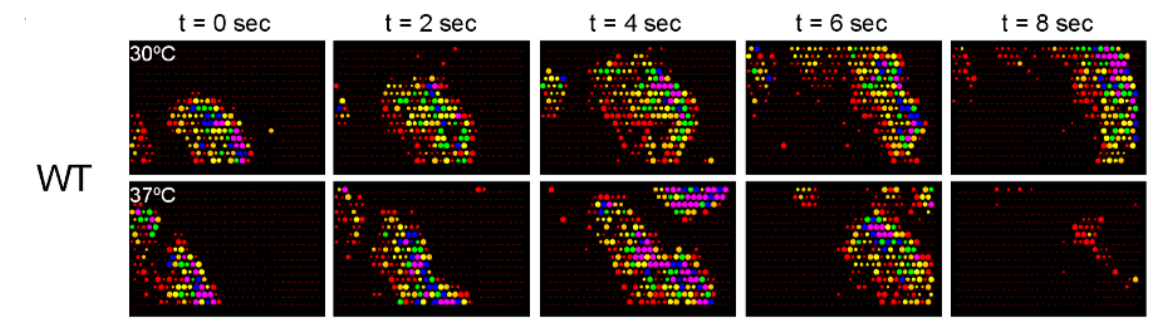
\includegraphics[width = \textwidth]{images/introduction/meaWaves}
	\def\c{Transient snapshots from the retina of a mouse placed on an MEA recorded at P6; the firing note is denoted by colour. }
	\caption[\c]{\label{fig:wtwaves} \c The waves are highly structured and propagate across the retina with the highest firing rates typically at the crest of the wave front. Figure adapted from Stafford et. al. (2009) \cite{Stafford2009}.}
\end{figure}
\subsubsection{$\beta2$  Knock-Out}
A genetic line of mouse has been generated which lacks the nicotinic-acetylcholine receptor $\beta2$ which shall henceforth be referred to as $\beta2$ knockout or just $\beta2^{-/-}$. The effect of the knock-out is a modification of the spatio-temporal characteristics of the waves. Initially it was thought to completely suppress activity leading to a low-correlation between any two given cells \cite{McLaughlin2003-yy}. This turned out to be a temperature based artefact and experiments confirm that it actually generates very fast spreading waves leading to a hyper-correlation between any two given retinal cells \cite{Stafford2009}; see Figure \ref{fig:beta2mea}. The effect of the $\beta2^{-/-}$ is to reduce the precision of the resulting topographic map: the receptive field of a given SC location is large with respect to wild-type \cite{Mrsic-Flogel2005-xp, McLaughlin2003-yy, Chandrasekaran2005-ug}.
\begin{figure}
	\begin{subfigure}{0.6\textwidth}
		\centering
		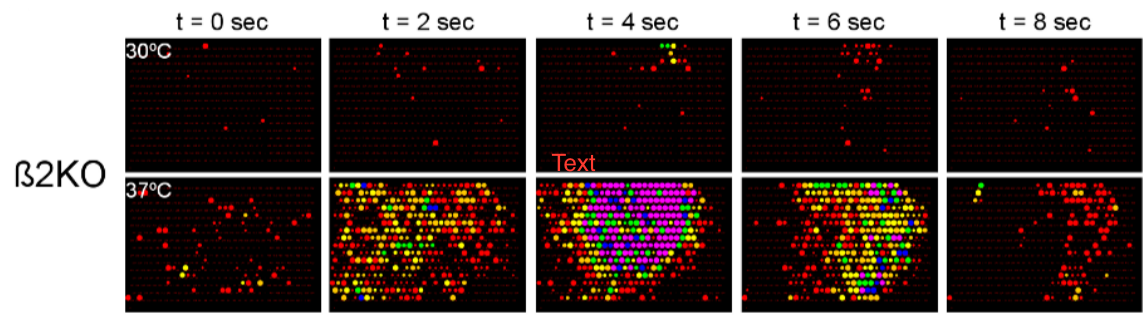
\includegraphics[width = \textwidth]{images/introduction/meaBeta2}
	\end{subfigure}
	~
	\begin{subfigure}{ 0.4\textwidth}
		\centering
		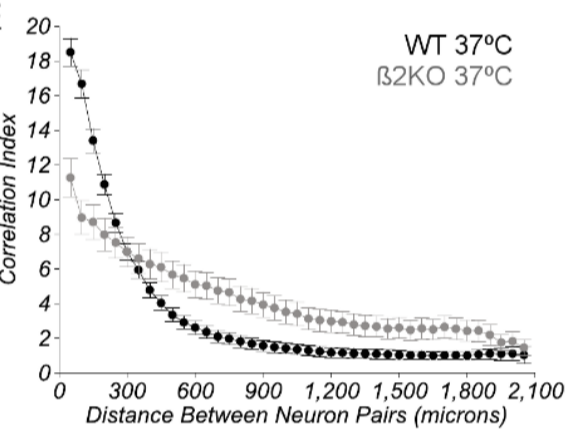
\includegraphics[width = \textwidth]{images/introduction/betacorrelation}
	\end{subfigure}

	\def\c{MEA recordings and correlational profile of retinal waves in the $\beta2^{-/-}$ mouse. }
	\caption[\c]{\label{fig:beta2mea} Transient snapshots from the retina of a $\beta2^{-/-}$ knock-out mouse placed on an MEA and recorded at P6 are shown in the left panel (a). The waves at normal body temperature are highly structured and propagate across the retina quickly and at high firing rates indicating a strong correlation between distal retinal locations. There is barely any activity at a cool temperature of 30C. Figure adapted from Stafford et. al. (2009) \cite{Stafford2009}.
	\\\\
	A measure of correlation is calculated as a function of distance and displayed in the right panel (b). The correlation is strongest for close wild-type pairs and drops off exponentially with a small length scale. For $\beta2^{-/-}$ knock-outs the correlation appears have a longer length scale indicating a hyper-correlation between distant retinal pairs.}
\end{figure}

\subsection{$Math5^{-/-}$ mutant}
The afferent incoming neurons are densely packed necessitating local interaction. They can interact directly with each other via chemical signalling, electrical signalling, or mechanical signalling. They indirectly interact by placing demands on the physical target structure such as metabolic demands of supporting dendritic contacts or physical space constraints. The role of competitive sorting is alluded to by the EphA3 knock-ins which are thought to separate their projections on the basis of relative sorting for which they need to competitively interact \cite{Reber2004-wq, Brown2000-da}. 

The aggregate effects of competitive interactions can be more directly deduced by reducing the number of interacting elements and this was examined in the $Math5$ knock-down \cite{Triplett2011-jk}. The effect of the knock-down was to reduce the number of RGCs born by 95\% distributed randomly across the retina. The substantially reduced number of incoming contacts resulted in a projection isolated to the anterior-medial region of the colliculus; see Figure \ref{fig:math5}.

\begin{figure}
	\centering
	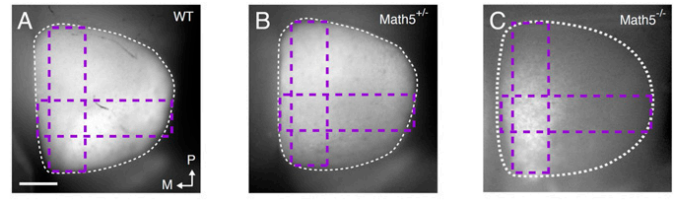
\includegraphics[width = 0.9\textwidth]{images/introduction/math5}
	\def\c{A full retina DiI injection revealing the entire image of the retinal projection on the SC. }
	\caption[\c]{\label{fig:math5} \c The wild-type and $Math5$ single knock-out (A and B) have normal RGC expression. The $Math5$ double knock-out supresses 95\% of RGC cells and subsequently only fills a portion of the anterior-medial colliculus (C). It is important to note that these studies do not show any topographic ordering as the entire colliculus is flooded with the tracer injections. Figure adapted from Triplett et. al. (2011) \cite{Triplett2011-jk}.}
\end{figure}

\FloatBarrier
\section{Developmental Theory  \label{section:developmentaltheory}}
Theoretical considerations have been useful and informative in guiding experimental work on the retinotopic projection with its successful implementation being attributed to a plurality of models and hypotheses guiding and clarifying experimental results \cite{Goodhill2018-ca}. The modelling literature will be examined shortly but the above data can be summarised into the unifying of three historical developmental narratives: the chemo-affinity hypothesis, the activity driven hypothesis, and the competitive sorting hypothesis.

\subsection{Competitive Hypothesis}
The competitive sorting hypothesis is, in essence, very simple working on the assumption that a specific location in the target area can only support a certain amount of synaptic contacts. Each retinal afferent is assumed to have some ability to compete for desirable space in the target area and the ability to compete is graded in some fashion: two common hypotheses were monotonically increasing chemical labels across the dimensions of the retina and time-of-arrival \cite{Prestige1975-vh, jacobson1960studies, Gaze1960-hw}. While evidence suggests chemically graded matching is the true mechanism, time-of-arrival allows discussion of competition without reference to an already discussed developmental mechanism. It states that each retinal point has a distinct location from which it departs and a unique time of arrival based on its time of neurogenesis. The first to arrive will be the first to place contacts and out-compete other incoming retinal afferents. Therefore, a smooth neighbourhood preserving map is formed by temporal differences in arrival of afferents related to the geometric distances between them. Thus, topography is established. This method of establishing topography is extremely sensitive to perturbation; any disruption in the initial ordering will lead to a disruption in the map. These considerations imply that competition with some biasing signal can provide a sorting method to establish topography and which is robust with a persistent bias, as is the case with chemotactic cues, and unstable with a non-persistent bias, such as time-of-arrival.
\subsection{Chemo-affinity Hypothesis \label{section:chemohypothesis}}
The chemo-affinity hypothesis was first proposed by Sperry and is essentially summarised as a mass-action rule: the position of an incoming afferent will be where the equilibrium point of repulsive or attractive chemical forces exists in the post-synaptic target \cite{Sperry1963-jc}. With a monotonic graded chemical distribution in both the pre-synaptic and post-synaptic areas this equilibrium point was proposed to be unique enabling topographic mapping. There is an immediate problem with the initial theory in that if both the pre-synaptic and post-synaptic targets have only one gradient then there is no native equilibrium point. This can be resolved in the first instance by tacitly introducing competitive mechanisms: each afferent will attempt to migrate towards the boundary but those expressing the highest levels of chemical guidance cue will dominate the boundary first with successively lower expression levels occupying successively interior points until a graded match is formed. This has been referred to as a Type I or graded matching mechanism \cite{Hjorth2015-le}. An alternative mechanism would be to introduce a counter-gradient in both directions with opposing interactions thereby establishing a natural equilibrium point where the two forces balance. This has been referred to as a Type II or `lock-and-key' mechanism \cite{Hjorth2015-le}. This mechanism only establishes a smoothly graded topographic map in the target area when the gradients are perfectly matched \cite{Gierer1983-rm, Sterratt2013-ev}. It can be rectified by again introducing competitive mechanisms but in this instance on the target area itself; when each location in the target can only support a given number of synaptic contacts any slight mismatch in gradients will be normalised out \cite{Sterratt2013-ev, Prestige1975-vh}.

\subsection{Activity Driven Hypothesis}
The activity hypothesis is based largely on the Hebbian hypothesis of synaptic potentiation. Briefly, it states that neurons in the pre-synaptic target which have highly correlated patterns of firing activity in the post-synaptic target will increase the strength of the synapses between them \cite{Hebb1949-wr}. Conversely, if these patterns are anti-correlated the synaptic strength will be decreased and thus, a feed-back loop is established. This allows for the \textit{de novo} establishment of topography under the assumption of correlated driving activity in the pre-synaptic area; domains of dominance will naturally be established and these will be continuous by construction. Therefore, a mapping is created with the neighbourhood preserving property and thus topography is established. The major problem with this theory is that when postulated in integral form (as the Hebbian rule is largely assumed to operate) it is valid on domains almost everywhere i.e. there is a set of Lebesgue measure zero (1D) for which discontinuities are allowed. This has significant implications for biology as on this set of discontinuities the orientation of the map can be reversed. This problem, again, can be fixed by including a competitive mechanism. A complete orientation flip would imply that incoming afferents completely cross over each other at least as many times as there are discontinuities which is metabolically costly and physically demanding. If the afferents have to interact with each other they will favour aligned domains and if each individual domain is aligned then they will be continuous across the whole boundary thus establishing topography.

\subsection{Unified Mechanisms}
Each of these three broad mechanisms enjoy experimental support. The existence of the Eph-ephrin class of molecules with a gradient and counter-gradient along both axes strongly implies a chemotactic component with a Type II mechanism. The existence of a series of retinal waves which appear to encode natural visual-field statistics supports the notion of activity driving mechanisms. The effect of the $Math5$ knock-down shows that competitive interaction is essential lending support to all three.

The existence of competition is explained immediately as a corrective mechanism: it alone is too sensitive to random fluctuations to be a primary mechanism but in conjunction with either of the mechanisms it can correct perturbations and sensitivities. Bidirectional chemotaxis with competition seems to be a complete explanation but theoretical considerations about thermal noise and the ability of neurons to detect these molecules means that there is a limit to the precision of the map established \cite{Goodhill2016-ck}. Activity with competition can create a topographic map but it is completely degenerate with respect to rotational symmetry. Therefore, it cannot be relied on to establish a map with a given orientation which is essential when multiple maps need to coordinate inputs. It can however, be relied on to produce precise and well defined domains thus normalising projective/receptive fields at a given width defined by activity patterns. 

These consideration lead to the following explanation: the chemotactic mechanisms in conjunction with competition can establish a well oriented topographic map but are sensitive to a noise floor while detecting relative expression levels of Ephs and ephrins. This explains the large axonal arbours which are initially established in the target. The lock and key nature can be seen in the ephrinA knock-outs which disrupt location specific topographic order. The gradients are also not perfectly matched. In the data this is presented with the axonal overshoot as all afferents compete to reach the preferential boundary. It is further confirmed by the $Math5$ knock-down where only the region near the preferential boundary is occupied suggesting dominance of the gradient or counter-gradient. The activity mechanism is then used to prune the pre-established axonal arbours to a precision that is appropriate to the biological system by matching relevant visual field statistics with a pre-determined spontaneous activity input prior to eye opening.

